\documentclass[a4paper, openany, 12pt]{article}

\usepackage{amsthm}
\newtheorem{theorem}{Theorem}

%% подключаем стандарт библиографии
\bibliographystyle{gost71u}

%% для "Abstract" в классе book
% \newenvironment{abstract}{}{}
% \usepackage{abstract}

%% подключаем преамбулу: в ней содержится подключение всех необходимых пакетов
\input{include/preambule.tex}

\begin{document}
    %% титульник
    \begin{center}
    %% *название института*
    \large\textbf{Министерство образования и науки Российской Федерации \\
    Московский физико-технический институт (государственный
    университет)} \\
    \vspace{1cm}

    %% *факультет/физтех-школа*
    Физтех-школа прикладной математики и информатики \\

    %% *название базовой кафедры и лаборатории*
    %% в случае ненадобности можно удалить
    Кафедра распознавания изображений и обработки текста (РИОТ)\\

    \vspace{3em}

    Выпускная квалификационная работа бакалавра
\end{center}

\begin{center}
    \vspace{\fill}
    %% *название вашей работы*
    \LARGE{Аугментации в задаче распознавания рукописного текста}

    \vspace{\fill}
\end{center}


\begin{flushright}
    \textbf{Автор:} \\
    Студент 020 группы \\
    Курочкин Павел Сергеевич \\
    \vspace{2em}
    \textbf{Научный руководитель:} \\
    Упшинский Андрей Леонидович \\
    \vspace{2em}
\end{flushright}

\vspace{7em}

\begin{center}
    %% *лого*
    \includegraphics[width=100 pt]{MIPT_logo.jpg}\\
    Москва \the\year{}
\end{center}

%% выключаем отображение номера для этой страницы (титульник)
\thispagestyle{empty}

\newpage
\setcounter{page}{2}
\fancyfoot[c]{\thepage}
%% *надпись над верхним колонтинулом*
%% в случае ненадобности можно удалить
\fancyhead[L]{Аугментации в задаче распознавания рукописного текста}
\fancyhead[R]{}
    %% аннотоция
    \begin{abstract}

    \begin{center}
        \large{Аугментации в задаче распознавания рукописного текста} \\
    \large\textit{Курочкин Павел Сергеевич} \\[1 cm]

    В современных методах распознавания рукописного текста ключевым элементом является наличие обширного массива аннотированных данных. Однако, в случае ограниченности данных, эффективное применение методов аугментации становится критически важным для повышения точности моделей. Manifold Mixup \hyperlink{cite.Ver18}{[1]} - современный метод аугментации данных, он представляет собой подход, в котором объединяются два или более изображения или их признаковые карты для создания новых образцов данных. В данном исследовании предлагается метод адаптации Manifold Mixup для использования с подходами, основанными на Connectionist Temporal Classification \hyperlink{cite.Gra06}{[2]}, в контексте задачи распознавания рукописного текста. Проводится всестороннее исследование данного метода, анализируется его влияние на процесс обучения нейронной сети. Результаты исследования показывают значительное улучшение результатов распознавания текста при использовании Manifold Mixup.

    \vfill

    \textbf{Abstract} \\[1 cm]

    Augmentations in handwritten text recognition
    \end{center}

\end{abstract}
\newpage
    %% содержание
    \tableofcontents{}
    \newpage

    % \fontsize{14}{16}\selectfont
    \section{Введение}
\label{sec:Chapter0} \index{Chapter0}

Распознавание текста является важным этапом в большинстве приложений по анализу изображений документов. Оно позволяет автоматически получать доступ к информации, содержащейся на страницах. За последнее десятилетие произошло огромное улучшение систем распознавания рукописного текста, связанное с появлением новых подходов и архитектур \hyperlink{cite.Gra06}{[2]}, \hyperlink{cite.Vas17}{[3]}, \hyperlink{cite.Gra08}{[4]}, \hyperlink{cite.Bas14}{[5]}, \hyperlink{cite.Joa17}{[6]}, \hyperlink{cite.The17}{[7]}, \hyperlink{cite.Mas23}{[8]}.

\subsection{Проблема}

Использование современных методов нейронных сетей помогает решить проблему высокой стилистической гетерогенности рукописного текста. Однако для таких мощных моделей с большим количеством параметров требуется значительное количество аннотированных изображений для обучения. Было предложено несколько методов, позволяющих уменьшить необходимость аннотированных данных при обучении систем распознавания текста.

Во-первых, обучающий набор можно расширить, добавив синтетические изображения. Это можно сделать, используя рукописные шрифты \hyperlink{cite.Mur03}{[9]} или создавая изображения текстовых строк на основе индивидуально извлеченных изображений реальных букв \hyperlink{cite.She16}{[10]}. Кроме того, для создания рукописных текстов можно применять генеративно-состязательные сети \hyperlink{cite.Alo19}{[11]}. 

Также, при ограниченном объеме данных, необходимо бороться с проблемой переобучения. Для этого было предложено множество подходов к регуляризации, таких как weight decay, dropout \hyperlink{cite.Sut14}{[12]}, batch normalization \hyperlink{cite.Iof15}{[21]} или раннее прекращение обучения, которые могут быть использованы в процессе обучения сети.

Наконец, для увеличения разнообразия обучающего набора, улучшения обобщающей способности модели и снижения риска переобучения широко применяются методы аугментации данных. Изображения могут быть отражены горизонтально и вертикально, подвергнуты поворотам и угловым трансформациям, изменены по размеру и масштабу. Также возможно добавление шума, обрезка изображений, цветовые трансформации и искажения в различных формах \hyperlink{cite.Cur17}{[13]}, \hyperlink{cite.Bas14}{[5]}. Подробнее методы аугментации для задачи распознавания рукописного текста описаны в \hyperref[sec:Chapter2]{Глава 3}.

В \hyperlink{cite.Cha11}{[14]} для создания новых обьектов было предложено интерполировать признаки обьектов одного класса. В \hyperlink{cite.Dev17}{[15]} было предложено использовать данный подход для признаков обьектов на выходе промежуточного слоя нейронной сети. В \hyperlink{cite.Ver18}{[1]} объединяются обе эти идеи и предлагается смешивать целевую переменную и изображения из разных классов, или их промежуточные признаки на различных уровнях сети. Последний подход показывают значительное улучшение качества на новых и состязательных данных. В \hyperlink{cite.Bas19}{[16]} представлен способ адаптации данного подхода для работы с решениями, основанными на Connectionist Temporal Classification \hyperlink{cite.Gra06}{[2]}. Последний подход был назван Manifold Mixup. 

Цель данного исследования заключается в анализе методов аугментации изображений в контексте распознавания рукописного текста и более детальном рассмотрении различных аспектов метода Manifold Mixup. Выбор использования Manifold Mixup обоснован следующими уникальными характеристиками данного метода:
\begin{enumerate}
\item Его легкость в обобщении на широкий спектр задач компьютерного зрения, решаемых с помощью нейронных сетей.
\item Согласно результатам исследований \hyperlink{cite.Ver18}{[1]}, \hyperlink{cite.Bas19}{[16]}, данный метод значительно способствует качеству и обобщенности обученной модели.
\end{enumerate}
 
\subsection{Постановка задачи}
Рассматриваемые методы аугментации изображений, включая метод Manifold Mixup \hyperlink{cite.Ver18}{[1]}, исследуемый в данной работе, предназначены для преодоления следующих проблем, возникающих в задаче распознавания рукописного текста:
\begin{enumerate}
\item Разнообразие изображений рукописного текста из-за различий в стилях авторов и фонах документов.
\item Недостаток аннотированных данных, что затрудняет обобщение моделей.
\item Риск переобучения из-за упомянутых выше проблем и большого количества параметров в сети.
\end{enumerate}
В данной статье проводится анализ различных методов агументаций, решающих данные проблемы. А также исследуются следующие аспекты метода Manifold Mixup:
\begin{enumerate}
\item Методы формирования батчей из изображений различных длин и их влияние на стабильность процесса обучения.
\item Роль выбора промежуточного слоя в процессе обучения для различных архитектур.
\item Влияние размера батча на обучение.
\item Воздействие Manifold Mixup на процесс обучения в зависимости от объема имеющихся данных.
\end{enumerate}

В \hyperref[sec:Chapter1]{Главe 2} приводится обзор существующих архитектур для решения задачи распознавания рукописного текста. Также представлена архитектура, применяемая в данном исследовании, обосновывается выбор данной архитектуры.


\hyperref[sec:Chapter2]{Глава 3} посвящена обзору существующих методов аугментации изображений для задачи распознавания рукописного текста, включая Manifold Mixup. Оценивается эффективность их применения для решения вышеупомянутых задач.

В \hyperref[sec:Chapter3]{Главe 4} представлено описание практической части и проведенных экспериментов.

\hyperref[sec:Chapter4]{Глава 5}  анализирует различные аспекты метода Manifold Mixup на основе проведенных экспериментов

И, наконец, в \hyperref[sec:Chapter5]{Главе 6} содержатся выводы из проведенного исследования.

\newpage %% fsd
    \section{Архитектура решения}
\label{sec:Chapter1} \index{Chapter1}

\begin{figure}
    \centering
    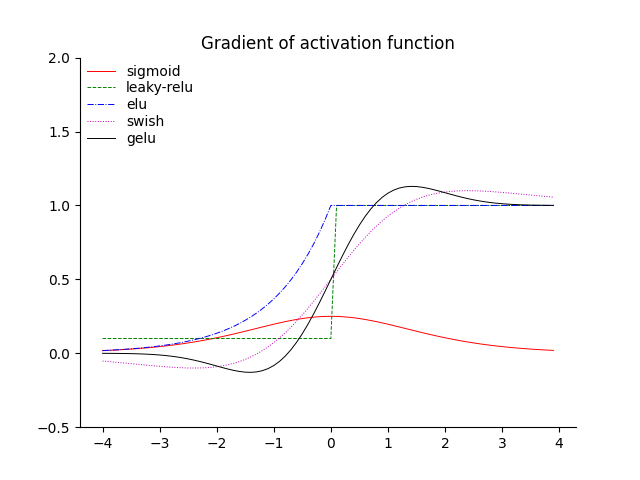
\includegraphics[scale=0.8]{./images/activation-funs-grad.png}
    \caption{\protect\hypertarget{image1}{Градиенты некоторых популярных функций активации.}}
\end{figure}


Современные модели, применяемые в задаче распознавания рукописного текста, обычно включают в себя три ключевых компонента:
\begin{enumerate}
\item Сверточную нейронную сеть, используемую для извлечения признаков из входных данных
\item Энкодер последовательности визуальных признаков
\item Декодер, который завершает процесс, трансформируя закодированные данные в окончательную текстовую транскрипцию
\end{enumerate}

\subsection{Извлечение визуальных признаков с помощью сверточной сети}
Подобно другим задачам компьютерного зрения, сверточная сеть используется для извлечения соответствующих визуальных признаков из текстовых изображений. Следующие архитектуры являются популярным выбором: ResNet \hyperlink{cite.Kai15}{[17]}, Inception \hyperlink{cite.Sze14}{[18]}, MobileNet \hyperlink{cite.San18}{[19]}. Увеличение сложности сверточной сети, как правило, приводит к умеренному приросту точности модели \hyperlink{cite.Her21}{[20]}. В этой работе используется архитектура ResNet. 

\newpage

\begin{figure}
    \centering
    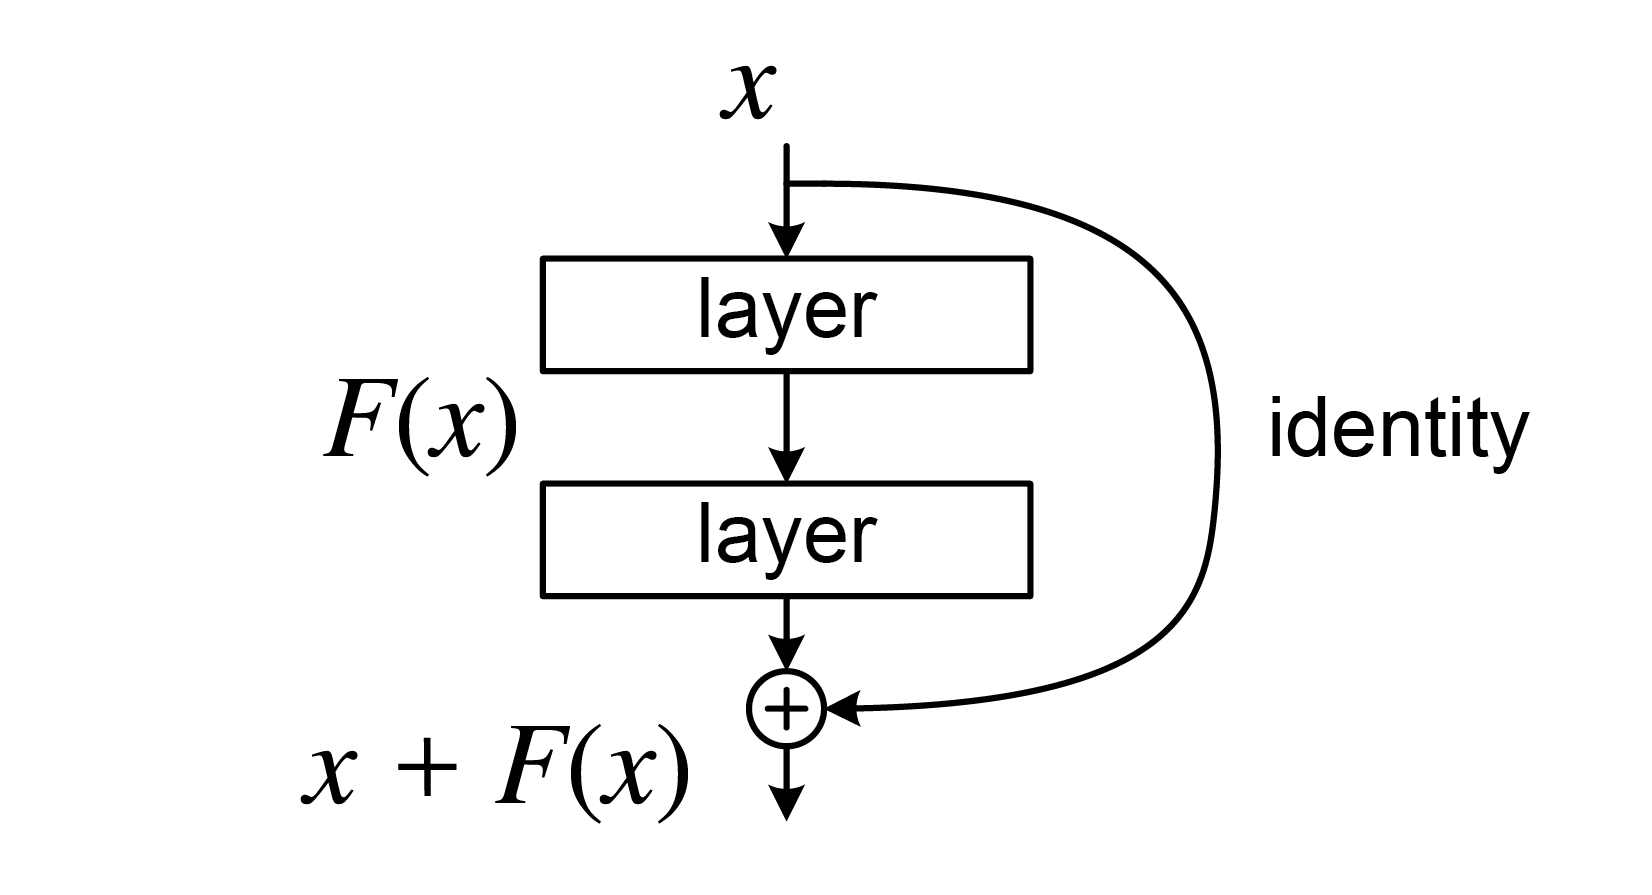
\includegraphics[scale=1]{./images/ResBlock.png}
    \caption{\protect\hypertarget{image2}{Residual блок.}}
\end{figure}

\subsubsection{Residual connection}
При обучении глубоких моделей градиент имеет тенденцию становиться очень маленьким: это называется проблема исчезающего градиента. Это связано с тем, что градиент проходит через ряд слоев, каждый из которых может уменьшить его. Например, градиент многих популярных функций активации приближается к нулю на значительной части числовой прямой \hyperlink{image1}{[Рис 1]}. 

Одним из решений проблемы исчезающего градиента является использование в качестве слоев нейронной сети residual блока \hyperlink{image2 }{[Рис 2]}, определенного следующим образом:
\begin{equation}
	\mathcal{F}_{l}^{'}(x) = \mathcal{F}_{l}(x) + x
\end{equation}
где $\mathcal{F}_{l}$ - стандартное нелинейное отображение (например, линейное - функция активации - линейное). Зачастую легче научиться предсказывать небольшое возмущение на входе, чем результат напрямую.

Модель с residual блоком имеет такое же количество параметров, как и модель без него, но ее легче тренировать. Причина в том, что градиенты могут перетекать непосредственно из выходных данных в более ранние слои. Чтобы убедиться в этом, рассмотрим градиент функции ошибки по параметрам слоя $l$. Имеем
\begin{equation}
	z_L = z_l + \sum_{i=l}^{L-1} \mathcal{F}_i(z_i ; \theta_i)
\end{equation}
где $z_i$ - признаки на выходе из $i$-го слоя сети. Таким образом, мы можем вычислить градиент функции потерь относительно параметров $l$-го слоя следующим образом:
\begin{equation}
	\frac{\partial \mathcal{L}}{\partial \theta_{l}} = 
	\frac{\partial z_{l}}{\partial \theta_{l}} \frac{\partial \mathcal{L}}{\partial z_{L}}
	(1 + \sum_{i=l}^{L-1} \frac{\partial \mathcal{F}_i(z_i; \theta_i)}{\partial z_{l}})
\end{equation}
Таким образом, мы видим, что градиент на слое $l$ напрямую зависит от градиента на слое $L$, причем независимо от глубины сети.
\begin{figure}
    \centering
    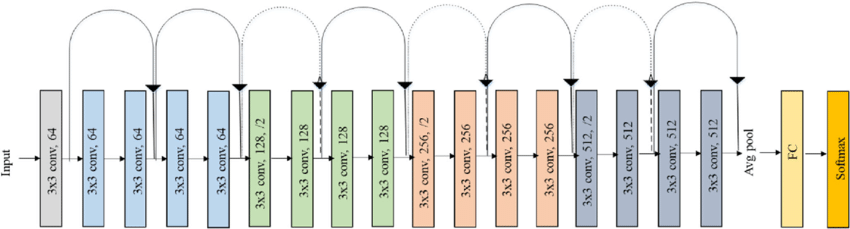
\includegraphics[scale=0.3]{./images/ResNet18.png}
    \caption{\protect\hypertarget{image3}{Архитектура ResNet-18.}}
\end{figure}

\newpage
\subsubsection{ResNet}
Победителем конкурса по компьютерному зрению \href{https://image-net.org/challenges/LSVRC/2015/}{ImageNet} 2015 года стала команда Microsoft, предложившая модель, известную сейчас как ResNet \hyperlink{image3}{[Рис 3]}. Данная модель состоит из residual блоков, имеющих следующий вид: свертка-BN-relu-свертка-BN, где BN - батч нормализация \hyperlink{cite.Iof15}{[21]}). Подобная архитектура позволяет обучать очень глубокие модели, а также решает проблему затухания градиентов. Именно из-за указанных преимуществ, а также из практического опыта, данная архитектура была отобрана для проведения данного исследования.

\begin{figure}
    \centering
    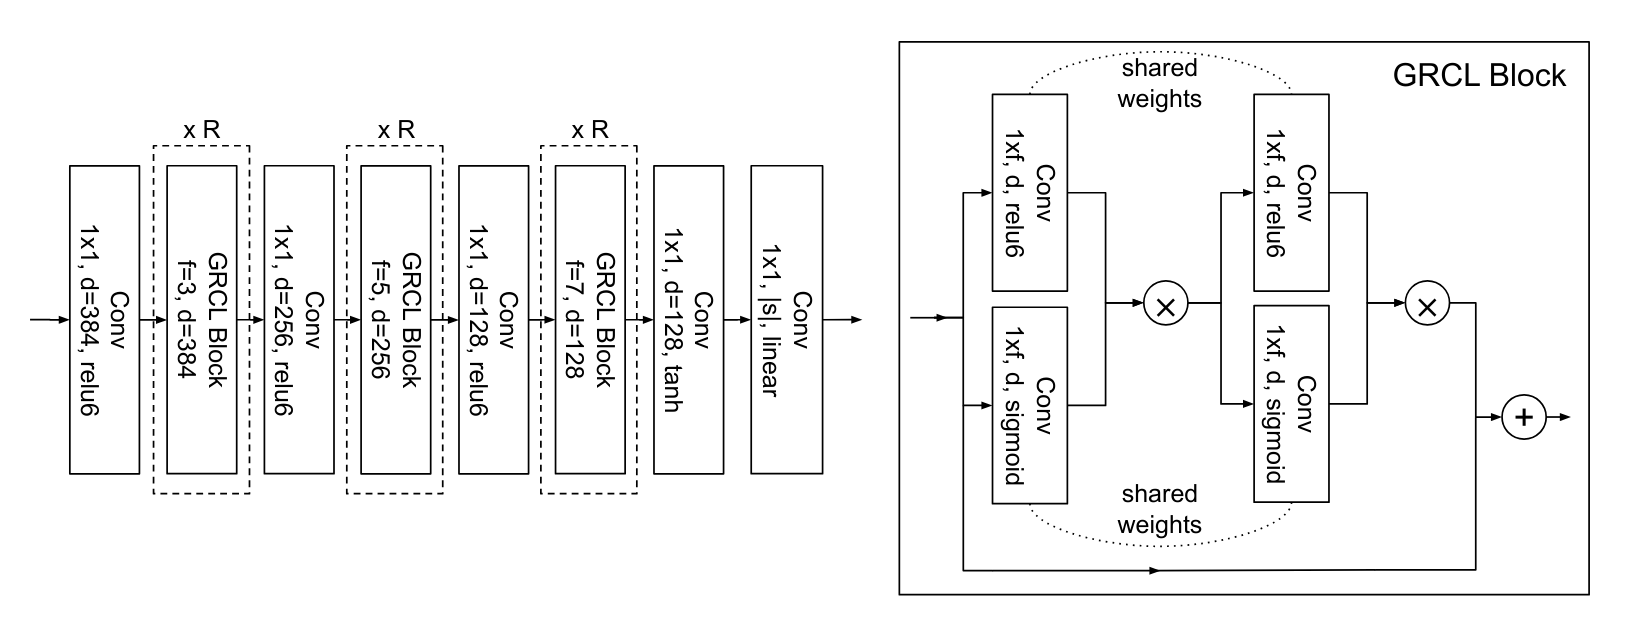
\includegraphics[scale=0.3]{./images/GRCL.png}
    \caption{\protect\hypertarget{image4}{Архитектура GRCL.}}
\end{figure}

\subsection{Энкодер последовательности визуальных признаков}
Сверточная сеть, предназначенная для извлечения визуальных признаков, имеет ограниченное рецептивное поле, что ограничивает ее способность учитывать широкий контекст информации. Это создает сложности при обработке длинных последовательностей в сложных сценариях, таких как распознавание рукописного текста. Для учета контекста на больших расстояниях используется энкодер. Существует много различных
архитектур энкодера, далее будут рассмотрены основные из них.

\subsubsection{Рекуррентные нейронные сети}
Рекуррентная нейронная сеть — это нейронная сеть, которая отображает входное пространство последовательности в выходное пространство последовательностей с сохранением состояния. То есть элемент выходной последовательности $y_t$ зависит не только от элемента входной последовательности $x_t$, но и от скрытого состояния системы $h_t$, которое обновляется. Для простоты обозначений пусть T будет длиной вывода (с учетом того, что она выбирается динамически). Тогда рекурентная сеть соответствует следующей условной генеративной модели:

\begin{equation}
	p(y_{1:T} | x) = \sum_{h_{1:T}} p(y_{1:T}, h_{1:T} | x) = \sum_{h_{1:T}} \prod_{t=1}^{T} p(y_{t} | h_{t})p(h_{t} | h_{t-1}, y_{t-1}, x)
\end{equation}
где $h_t$ — скрытое состояние, и где мы определяем $p(h_1 |h_0, y_0, x) = p(h_1 |x)$ как начальное скрытое состояние. Мы предполагаем, что скрытое состояние вычисляется детерминированно следующим образом:

\begin{equation}
	p(h_t | h_{t-1}, y_{t-1}, x) = \mathbb{I}(h_t = f (h_{t-1}, y_{t-1}, x)) 
\end{equation}
для некоторой детерминированной функции $f$. Функция обновления $f$ обычно задается выражением

\begin{equation}
	h_t = \varphi (W_{xh} [x; y_{t-1}] + W_{hh}h_{t-1} + b_h) 
\end{equation}

Рекурентные сети с достаточным количеством скрытых единиц в принципе могут запоминать входные данные из далекого прошлого. Однако сети с "ванильной" архитектурой не могут этого сделать из-за проблемы исчезающего градиента. Существует архитектурное решение данной проблемы, в котором мы обновляем скрытое состояние аддитивным способом, аналогично residual блокам в ResNet: GRU и LSTM.

Различные варианты рекуррентных сетей использовались для решения задачи распознавания рукпоисного текста: LSTM \hyperlink{cite.Bas14}{[5]} \hyperlink{cite.Gra08}{[4]}, BiLSTM \hyperlink{cite.The17}{[6]} \hyperlink{cite.Joa17}{[7]}, Gated Recurrent Convolution Layer (GRCL) \hyperlink{image4}{[Рис 4]} \hyperlink{cite.Lux17}{[22]}.

\begin{figure}
    \centering
    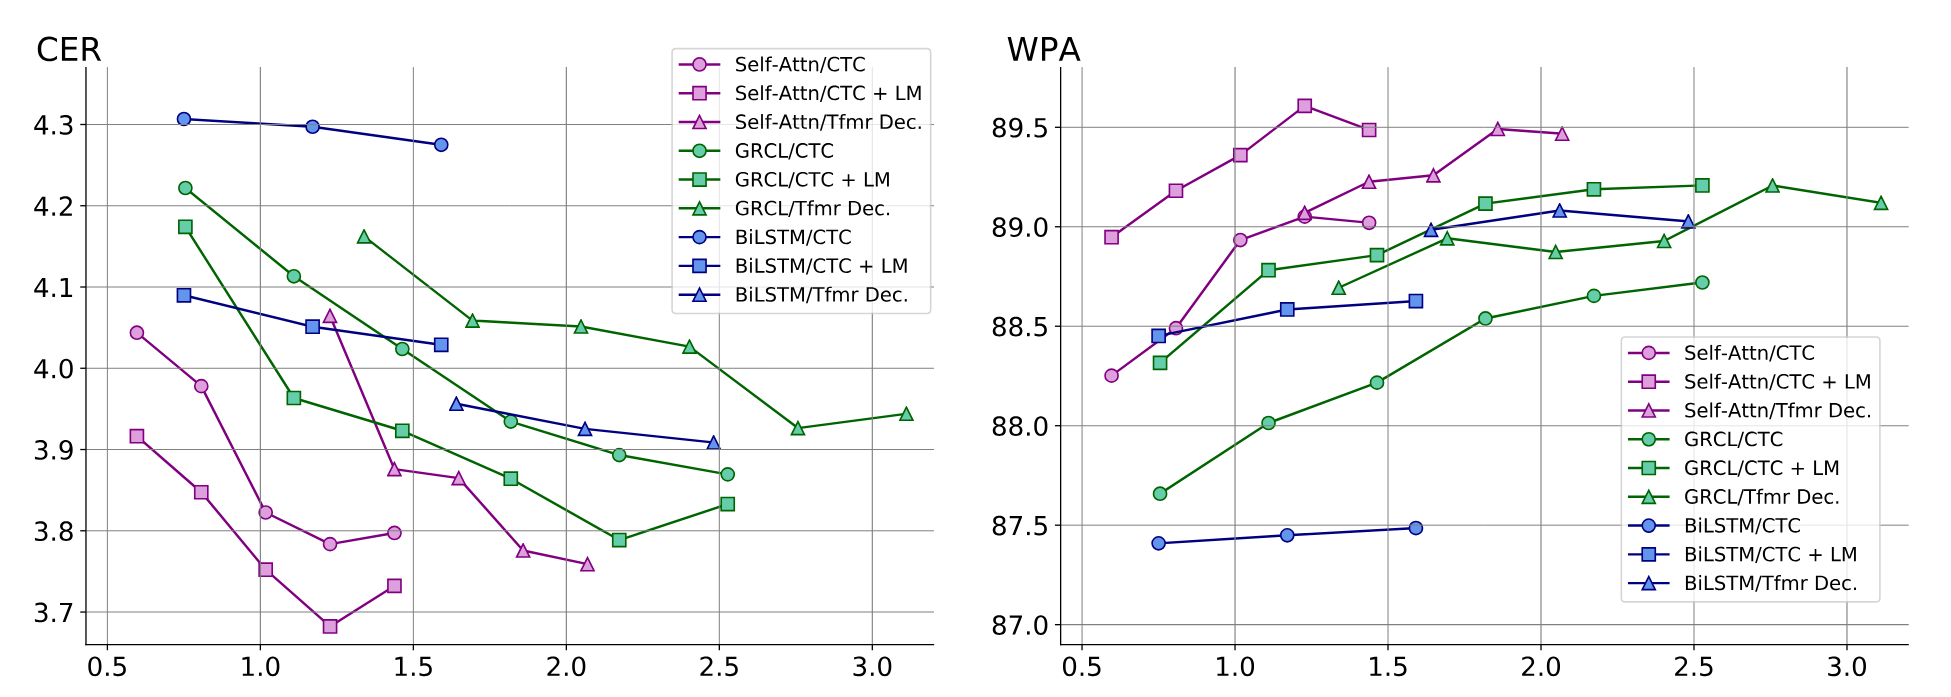
\includegraphics[scale=0.25]{./images/competition.png}
    \caption{\protect\hypertarget{image5}{Сравнение различных архитектур для задачи распознавания текста. \\ Взято из \protect\hyperlink{cite.Her21}{[20]}}.}
\end{figure}

\subsubsection{Self-Attention}
Self-Attention энкодер, предложенный в \hyperlink{cite.Vas17}{[3]} широко используется в задачах из NLP и компьютерного зрения. Распознавание текстовых строк, как задача преобразования изображения в последовательность, не является исключением. Self-attention способен улавливать долгосрочные зависимости в последовательностях лучше, чем рекуррентные сети, благодаря возможности обрабатывать взаимодействия между всеми элементами последовательности одновременно. Также, в отличие от рекуррентных сетей, self-attention не сталкивается с проблемой затухания градиентов.

Выход сверточной сети, с удаленным измерением высоты изображения ($X \in \mathbb{R} ^ {n \times d}$), поступает в энкодер. Выход $Y$ слоя Attention получается следующим образом:

\begin{equation}
\begin{split}
	Q = X W_q \\
	K = X W_k \\
	V = X W_v \\
	Y = softmax(\frac{Q K^T}{\sqrt{d}}V)
\end{split}
\end{equation}
где $W_q$, $W_k$ и $W_v$ — матрицы параметров размера $d \times d$, которые задают проекцию входной последовательности $X$ в пространство запросов, ключей и значений соответственно. Закодированный признак Y представляет собой выпуклую комбинацию вычисленных значений $V$, матрица  сходства вычисляется как скалярное произведение запросов и ключей.

Эффективность "ванильного" Attention может быть низкой, поскольку данный слой инвариантен к перестановкам, и, следовательно, игнорирует порядок элементов входной последовательности. Чтобы преодолеть эту проблему, к признакам элементов входной последовательности добавлятся информация о позиции элемента (positional embedding). Можно представить positional embedding как матрицу $\mathbf{P}^{n \times d}$.

В \hyperlink{cite.Vas17}{[3]} было предложено использовать синусоидальный базис следующего вида:
\begin{equation}
	p_{i,2j} = \sin(\frac{i}{C^{\frac{2j}{d}}}), \quad p_{i,2j+1} = \cos(\frac{i}{C^{\frac{2j}{d}}}) 
\end{equation}
где $C$ соответствует некоторой максимальной длине последовательности. Одним из важных плюсов данного представления является то, что представление одной позиции линейно предсказуемо относительно любой другой, если известно их относительное расстояние. В частности, выполняется $p_{t+ \phi} = f (p_t)$, где $f$ - некоторое линейное отображение. А именно
\begin{equation}
\begin{pmatrix}
	\sin(\omega_k (t + \phi)) \\
	\cos(\omega_k (t + \phi))
\end{pmatrix} = 
\begin{pmatrix}
	\cos (\omega_k \phi)  & \sin (\omega_k \phi) \\
	-\sin (\omega_k \phi) & \cos (\omega_k \phi)
\end{pmatrix}
\begin{pmatrix}
	\sin(\omega_k t) \\
	\cos(\omega_k t)
\end{pmatrix}
\end{equation}
То есть при маленьком $\phi$ имеем $p_{t + \phi} \approx p_t$. Positional embedding, как правило, прибавляется ко входу, то есть:
$PosEmbed(X) = X + \mathbf{P}$.

Существуют также другие варианты. Например, relative positional embedding \hyperlink{cite.Sha18}{[23]}.

\subsection{Метрики}
Пусть S - это набор обучающих примеров, выбранных из фиксированного распределения $D_{\mathcal{X} \times \mathcal{Z}}$. Пространство входных данных $\mathcal{X} = (\mathbb{R}^m)^*$ представляет собой множество всех последовательностей из $m$-мерных векторов вещественных чисел. Целевое пространство $\mathcal{Z} = L^*$ представляет собой множество всех последовательностей из (конечного) алфавита $L$. В общем случае, мы обозначаем элементы $L^*$ как последовательности символов. Каждый пример в S состоит из пары последовательностей $(x, z)$. Целевая последовательность $z = (z_1, z_2, ..., z_U)$ не длиннее входной последовательности $x = (x_1, x_2, ..., x_T)$, то есть $U \leq T$. Поскольку входные и целевые последовательности обычно не имеют одинаковой длины, нет априорного способа их выравнивания.

Цель состоит в использовании $S$ для обучения модели $h : \mathcal{X} \rightarrow \mathcal{Z}$, которая отображает последовательность признаков в последовательность символов таким образом, чтобы минимизировать некоторую специфическую ошибку задачи.

Общепризнанным выбором является следующая метрика: для заданного тестового набора $S_0 \subset D_{\mathcal{X} \times \mathcal{Z}}$, не пересекающегося с $S$, определяется коэффициент ошибок меток (label error rate, LER) модели $h$ как нормализованное расстояние Левенштейна между его предсказаниями и ответом на $S_0$, т.е.:
\begin{equation}
	LER(h, S_0) = \frac{\sum_{(x,z) \in S_0} ED(h(x), z)}{\sum_{(x,z) \in S_0} |z|}
\end{equation}
где $ED(p, q)$ - расстояние Левенштейна между двумя последовательностями $p$ и $q$, т.е. минимальное количество вставок, замен и удалений, необходимых для преобразования $p$ в $q$.
Это естественная метрика для задач (таких как распознавание речи или рукописного текста), где целью является минимизация частоты ошибок транскрипции. Популярными метриками в задаче распознавания рукописного текста являются WER (word error rate) и CER (character error rate) - описанное выше расстояние Левенштейна на уровне слов и символов соответственно.

Также в данном исследовании будет использоваться метрика LabelAccuracy (Label может быть словом, строкой или фрагментом). Определяется она так:
\begin{equation}
	LabelAcc(h, S_0) = 1 - LER(h, S_0)
\end{equation}


\subsection{Декодер}
Декодер завершает процесс, трансформируя закодированные данные в окончательную текстовую транскрипцию. В данном исследовании используется подход Connectionist Temporal Classification \hyperlink{cite.Gra06}{[2]}. Существуют также альтернативные модели: например, авторегрессионный декодер. 

\subsubsection{Авторегрессионный декодер}
В авторегрессионной модели значение токена в данный момент зависит от значений предыдущих токенов ряда. Для реализации такой модели обычно используют рекурентные сети или архитектуру Transformer \hyperlink{cite.Vas17}{[3]}. Например, Transformer стал предпочтительной архитектурой для задач прогнозирования последовательности, таких как машинный перевод. Он также широко применяется в задаче распознавания рукописного текста. Например, state-of-the-art решение согласно бенчмарку \href{https://paperswithcode.com/sota/handwritten-text-recognition-on-iam}{IAM} принадлежит на момент написания этого текста decoder-only transformer архитектуре \hyperlink{cite.Mas23}{[8]}. Минус данной архитектуры - это то, что она является более громоздкой. Она требует большего количества параметров и, соотвественно, данных для обучения \hyperlink{image5}{[Рис 5]}.

\begin{figure}
    \centering
    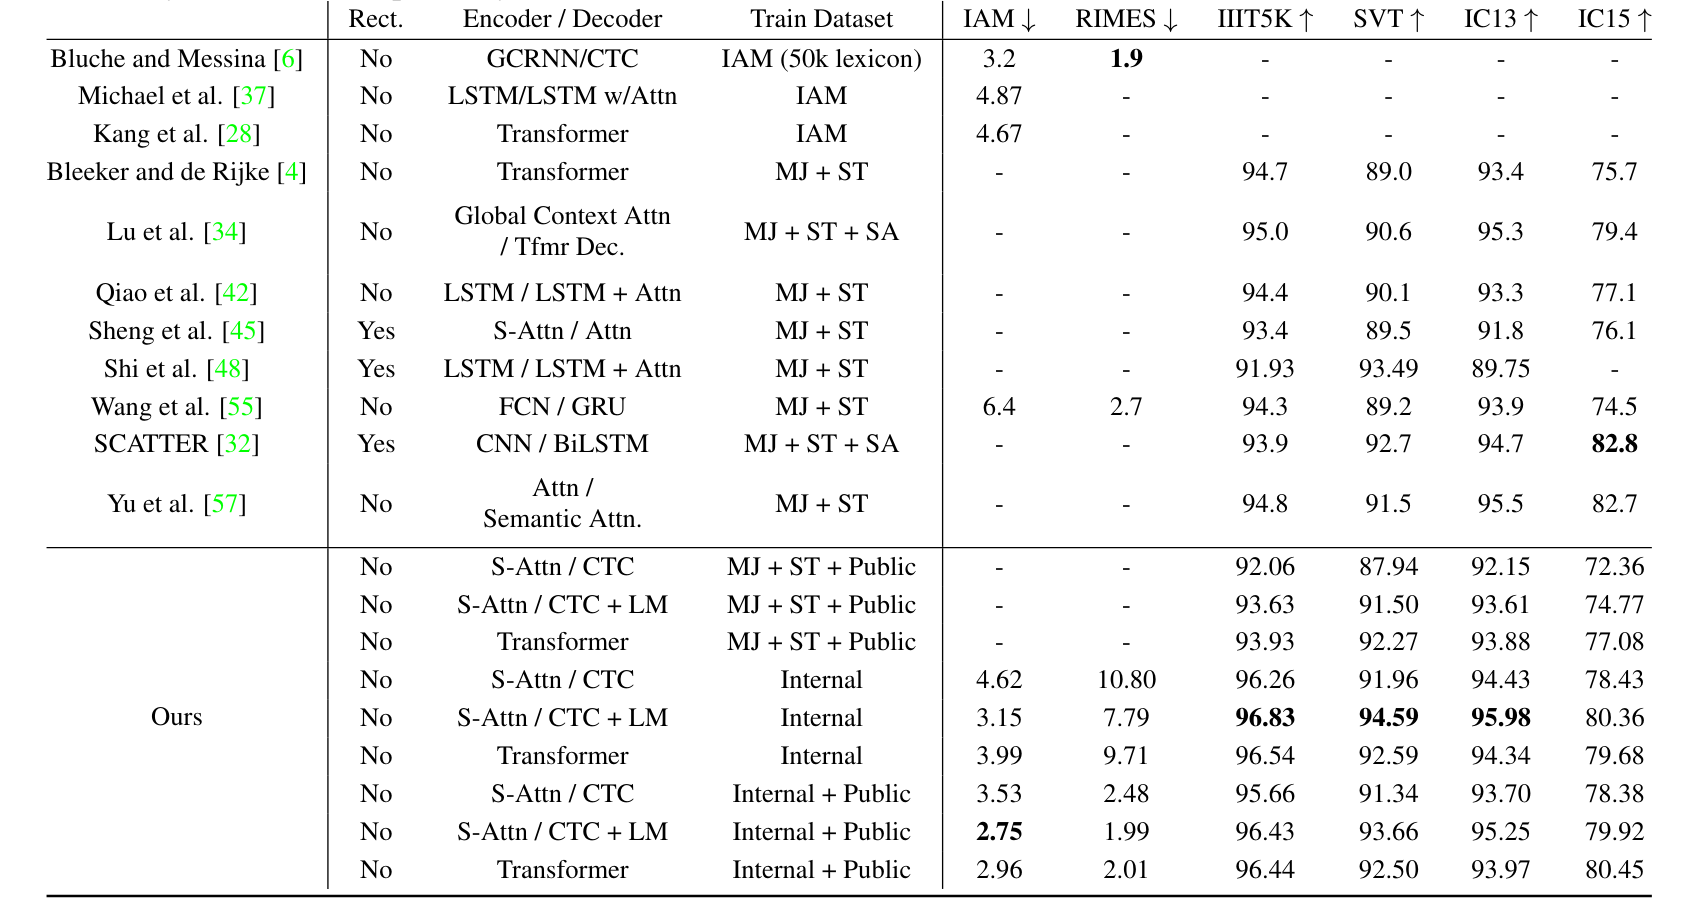
\includegraphics[scale=0.25]{./images/competition_all.png}
    \caption{\protect\hypertarget{image6}{Сравнение различных архитектур для задачи распознавания текста на различных бенмарках. \\ Взято из \protect\hyperlink{cite.Her21}{[20]}}.}
\end{figure}

\subsubsection{Connectionist Temporal Classification}
Декодер Connectionist Temporal Classification изначально использовался для распознавания речи, позже исследователи добились огромного успеха, применив его для задач распознавания текста.

Пусть мы имеем некоторую нейронную сеть $N_w : (\mathbb{R}^m)^T \rightarrow (\mathbb{R}^n)^T$. Пусть $y = N_w(x)$ - последовательность выходов сети, и обозначим $y_t^k$ активацию выходного узла $k$ в момент времени $t$ (последний слой softmax). Тогда $y_t^k$ интерпретируется как вероятность наблюдения символа $k$ в момент времени $t$, что определяет распределение над множеством $L_{0}^T$ длины $T$ последовательностей алфавита $L_0 = L \cup \{blank\}$. Тут мы добавляем в алфавит символ $blank$, обозначающий пропуск. Элементы $L_0^T$ обычно называют путями.

\begin{equation}
	p(\pi|x) = \prod_{t=1}^{T} y_t^{\pi_t}, \quad \forall \pi \in L_{0}^{T}
\end{equation}

Далее определим отображение $B: L_{0}^T \rightarrow L_{\leq T}$, где $L_{\leq T}$ - это множество последовательностей длиной менее или равной $T$ по оригинальному алфавиту $L$. Мы делаем это, просто удаляя все blank и повторяющиеся символы из путей. Интуитивно это соответствует выводу нового символа, когда сеть переходит от предсказания отсутствия символа к предсказанию символа, или от предсказания одного символа к другому. Наконец, используем $B$ для определения условной вероятности данного предсказания $I \in L_{\leq T}$ как сумму вероятностей всех путей, соответствующих ему:
\begin{equation}
	p(I|x) = \sum_{\pi \in B^{-1}(I)} p(\pi|x)
\end{equation}

Вывод классификатора должен быть наиболее вероятным предсказанием для входной последовательности:
\begin{equation}
	h(x) = \arg\max_{I \in L_{\leq T}} p(I|x)
\end{equation}

В данном исследовании поиск такого предсказания строится на предположении, что наиболее вероятный путь будет соответствовать наиболее вероятному предсказанию:
\begin{equation}
\begin{split}
	h(x) \approx B(\pi^{*}) \\
	\pi^{*} = \arg\max_{\pi \in L_0^T} p(\pi|x).
\end{split}
\end{equation}
Это легко найти, так как $\pi^{*}$ представляет собой просто конкатенацию самых вероятных символов на каждом этапе. Такой подход не гарантирует нахождение наиболее вероятного предсказания, но достаточно хорошо его приближает. 

Модель обучается методом максимального правдоподобия. Для вычисления условных вероятностей $p(I|x)$ отдельных предсказаний используется динамическое программирование \hyperlink{cite.Gra06}{[2]}. Также включение явной языковой модели поверх логитов может значительно повысить точность \hyperlink{cite.Fuj17}{[24]}.
\paragraph{}
Во время выбора архитектуры учитывался собственный практический опыт, а также результаты исследований по данной теме. Например, в \hyperlink{cite.Her21}{[20]} проводится сравнительный анализ различных архитектур энкодеров / декодеров \hyperlink{image6}{[Рис 6]}. Было решено выбрать в качестве:
\begin{enumerate}
\item Сверточной нейронной сети: ResNet
\item Последовательного энкодера: TransformerEncoder
\item Декодера: Connectionist Temporal Classification
\end{enumerate}

\newpage %% Постановка задачи
    \section{Обзор существующих методов аугментации изображений для задачи распознавания рукописного текста}
\label{sec:Chapter2} \index{Chapter2}

\begin{figure}
    \centering
    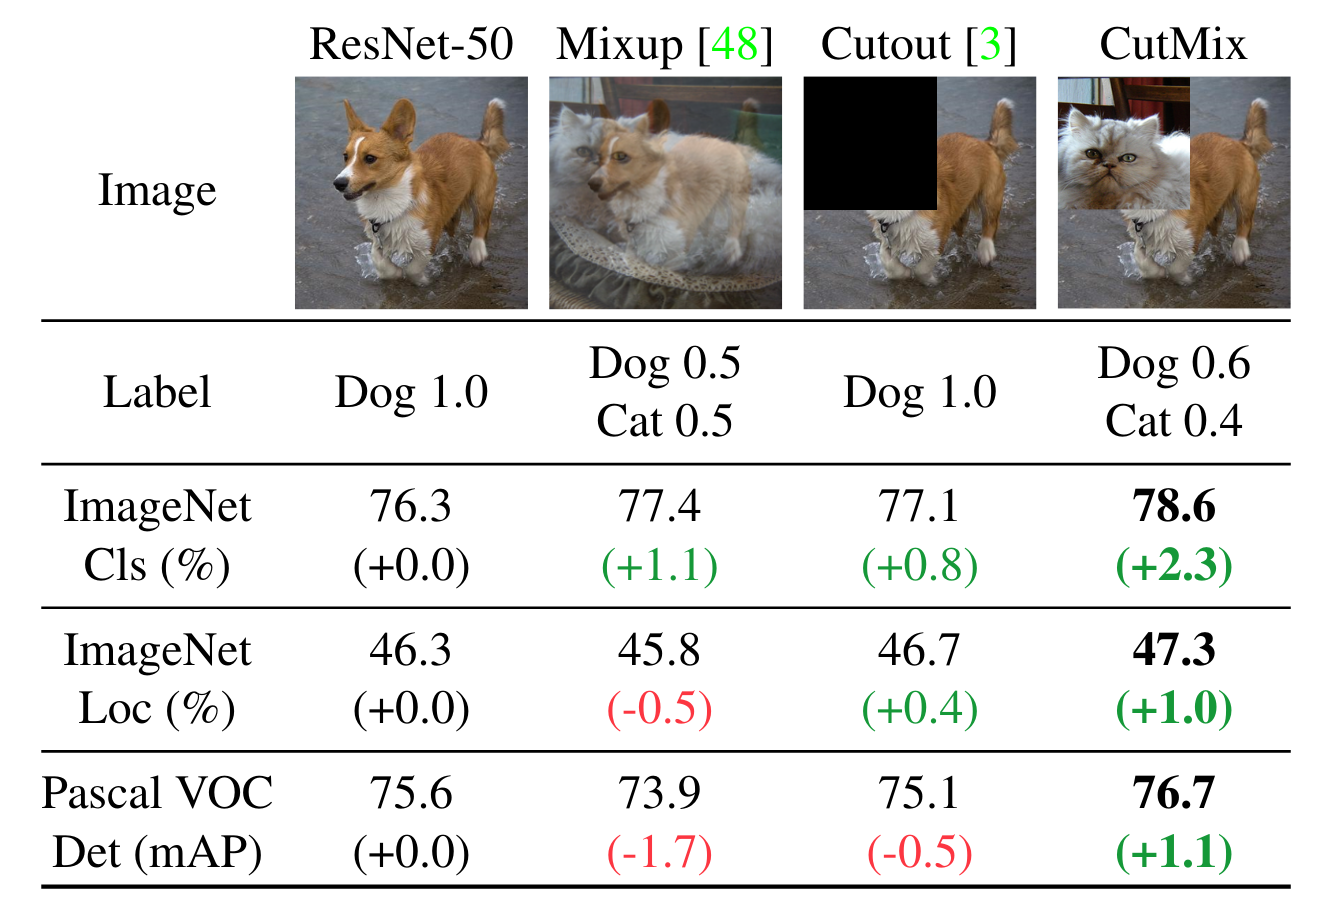
\includegraphics[scale=0.25]{./images/cutmix.png}
    \caption{\protect\hypertarget{image7}{Результаты различных техник аугментаций на ImageNet. \\ Взято из \protect\hyperlink{cite.Yun19}{[26]}}.}
\end{figure}

Помимо распространенных техник аугментации, которые используются в широком спектре задач компьютерного зрения, таких как:
\begin{enumerate}
\item отражение по горизонтали/вертикали,
\item повороты и угловые трансформации,
\item изменение масштаба,
\item добавление шума,
\item обрезка,
\item цветовые преобразования,
\item искажения различных форм,
\end{enumerate}
существуют также методы аугментации, которые специфически применяются для решения определенных задач. Далее будут описаны некоторые из таких методов аугментации. В каждом из рассмотренных видов аугментации новые объекты создаются путем комбинирования двух или более объектов из набора данных.

\subsection{CutMix}
Пусть $x \in \mathbb{R}^{W \times H \times C}$ и $y$ обозначают изображение и его целевую переменную соответственно. Целью метода CutMix является создание нового образца $(\tilde{x}, \tilde{y})$ путем комбинирования двух образцов $(x_A, y_A)$ и $(x_B, y_B)$. \hyperlink{image7}{[Рис 7.]} Созданный образец $(\tilde{x}, \tilde{y})$ используется для обучения модели с использованием ее исходной функции потерь. Операция комбинирования определяется следующим образом:
\begin{equation}
\begin{split}
\tilde{x} = M \odot x_A + (1 - M) \odot x_B \\
\tilde{y} = \lambda y_A + (1 - \lambda) y_B,
\end{split}
\end{equation}
где $M \in {0, 1}^{W \times H}$ обозначает бинарную маску, $1$ - бинарная маска, заполненная единицами, и $\odot$ - покомпонентное умножение. $\lambda$ выбирается из бета-распределения $Beta(\alpha, \alpha)$. В отличие от mixup \hyperlink{cite.Hon17}{[25]}, CutMix \hyperlink{cite.Yun19}{[26]} заменяет область изображения патчем из другого обучающего изображения и создает более локально естественное изображение.

Для выборки бинарной маски $M$ мы сначала выбираем координаты ограничивающего прямоугольника $B = (r_x, r_y, r_w, r_h)$. Область $B$ в $x_A$ удаляется и заполняется частью, обрезанной из $B$ на $x_B$. Выбираются прямоугольные маски M, соотношение сторон которых пропорционально оригинальному изображению. Координаты прямоугольников выбираются равномерно в соответствии со следующим правилом:
\begin{equation}
\begin{split}
r_x \sim Unif (0, W), r_w = W \sqrt{1 - \lambda} \\
r_y \sim Unif (0, H), r_h = H \sqrt{1 - \lambda}
\end{split}
\end{equation}
соотношение площадей картинок есть 
\begin{equation}
\frac{r_w r_h}{WH} = 1 - \lambda
\end{equation}
На каждой итерации обучения CutMix-образец ($\tilde{x}, \tilde{y}$) генерируется путем комбинирования случайно выбранных двух образцов в батче.

\begin{figure}
    \centering
    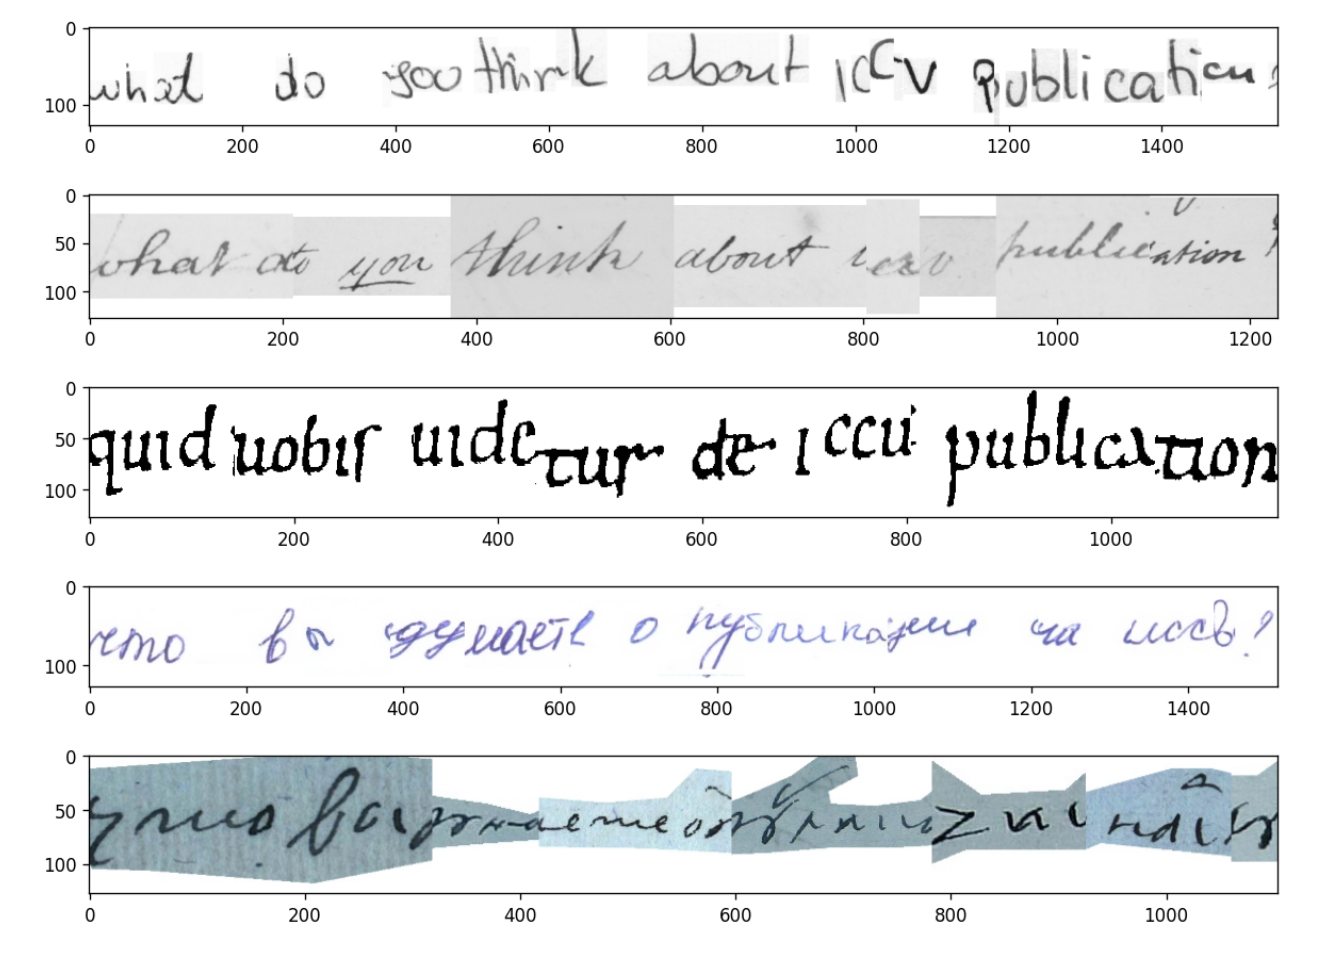
\includegraphics[scale=0.25]{./images/stackmix.png}
    \caption{\protect\hypertarget{image8}{Примеры изображений, созданных с помощью StackMix. \\ Взято из \protect\hyperlink{cite.Sho21}{[27]}.}}
\end{figure}

\subsubsection{StackMix}
В \hyperlink{cite.Sho21}{[27]} этот подход был адаптирован для задачи распознавания рукописного текста. В StackMix различные фрагменты рукописного текста склеиваются в некотором порядке. \hyperlink{image8}{[Рис 8.]}

Чтобы применить предложенный подход к задаче распознавания рукописного текста, требуется дополнительная разметка данных, которая точно отмечает границы символов. Для достижения этой цели используется подход с автоматической сегментацией обучающих изображений на символы с использованием постобработки контролируемой предварительно обученной нейронной сети (с декодером Connectionist Temporal Classification). 

\begin{figure}
    \centering
    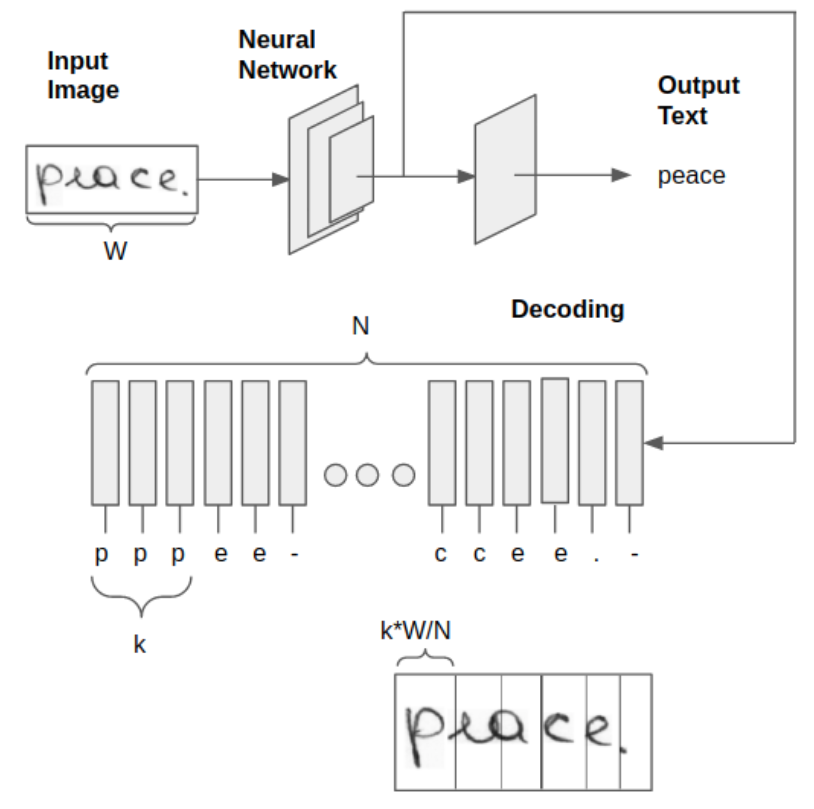
\includegraphics[scale=0.25]{./images/stackmix_algo.png}
    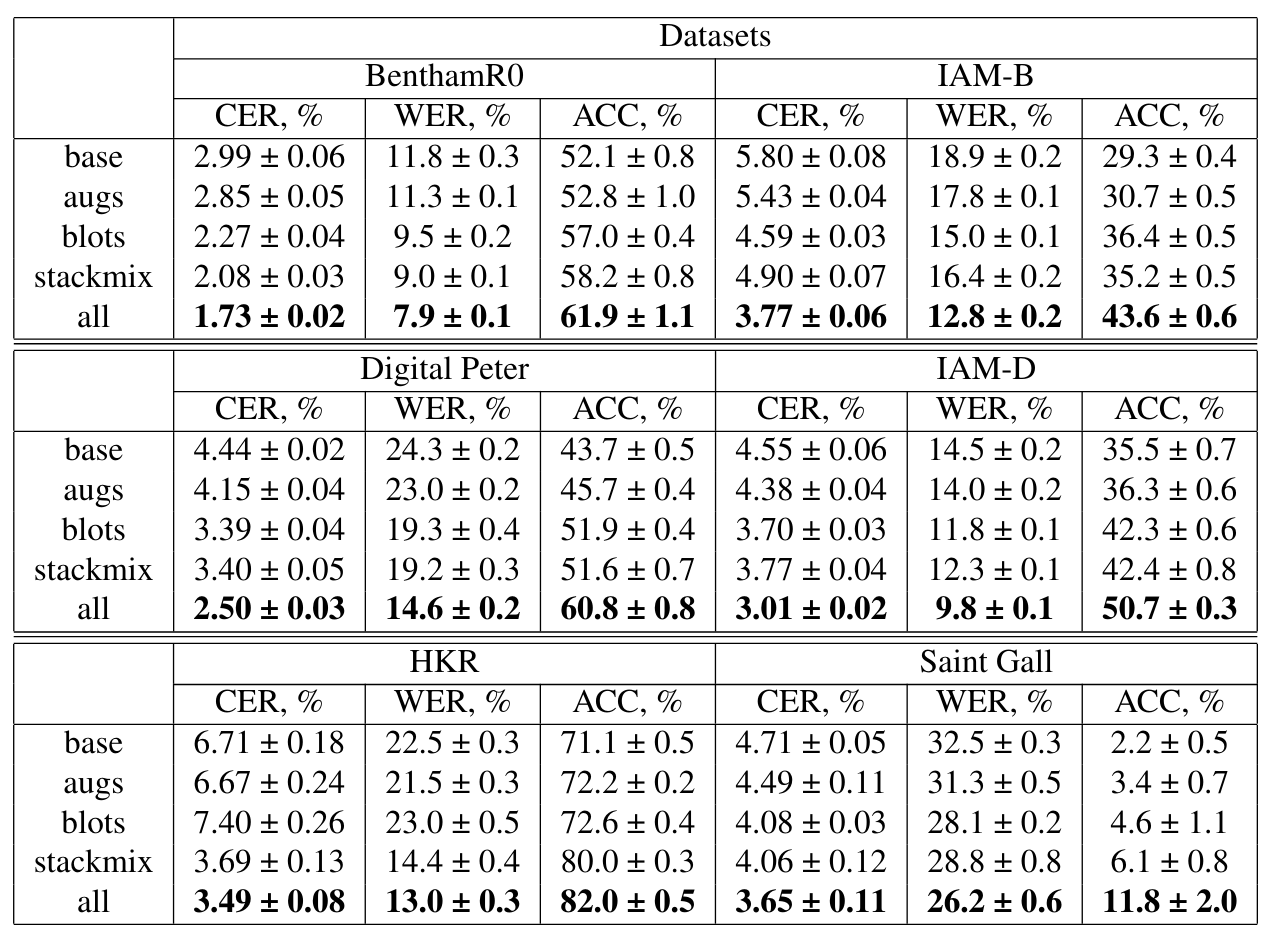
\includegraphics[scale=0.2]{./images/stackmix_results.png}
    \caption{\protect\hypertarget{image9}{Схема постобработки для получения границ символов в StackMix. А также результаты работы. \\ Взято из \protect\hyperlink{cite.Sho21}{[27]}.}}
\end{figure}

Основная идея заключалась в том, чтобы соединить последний слой RNN (после применения активации softmax для каждого символа из функций изображения) и ширину изображения, чтобы получить границы символов, используя только слабо контролируемое обучение без какой-либо ручной разметки \hyperlink{image9}{[Рис 9.]}. Для обучения нейронной сети можно использовать базовую схему без каких-либо дополнений и ухищрений. Для получения качественной разметки границ символов необходимо использовать выборку с этапа обучения.

Один из недостатков данного метода состоит в сильной зависимости от качества алгоритма, определяющего границы символов. Сгенерированные образцы отличаются именно в местах "склейки". В \hyperlink{cite.Sho21}{[27]} одним из свойств датасетов является четкость границы между символами в среднем (это было замечено эмпирически после их анализа). Однако не все рукописные тексты обладают таким качеством.

\subsection{Mixup}

В данном методе предлагается создавать новый образец ($\tilde{x}, \tilde{y}$) следующим образом:
\begin{equation}
\begin{split}
\tilde{x} = \lambda x_i + (1 - \lambda) x_j \\
\tilde{y} = \lambda y_i + (1 - \lambda) y_j
\end{split}
\end{equation}
где $(x_i, y_i)$ и $(x_j, y_j)$ - это два пары ($x$ - вектор признаков, $y$ - целевой объект), выбранные случайным образом из обучающих данных, а $\lambda \sim Beta(\alpha, \alpha), \alpha \in (0, \infty), \lambda \in [0, 1]$. Гиперпараметр $\alpha$ контролирует силу интерполяции между парами признаков-целевых объектов.

Mixup можно понимать как форму аугментации, которая побуждает модель вести себя линейно между по обучающим примерам. Утверждается, что такое линейное поведение уменьшает количество нежелательных колебаний при прогнозировании вне обучающих примеров. Обощением этой идеи является manifold mixup.

\subsubsection{Manifold mixup}

В \hyperlink{cite.Ver18}{[1]} исследователи обнаружили несколько свойств, касающихся скрытых представлений и границ решений современных нейронных сетей. Во-первых, граница решения часто резкая и близка к данным. Во-вторых подавляющая часть пространства признаков соответствует предсказаниям с высокой степенью достоверности, как внутри, так и вне многообразия данных. Руководствуясь этими интуициями, был придуман Manifold Mixup: простой регуляризатор, который устраняет некоторые из этих недостатков путем обучения нейронных сетей на линейных комбинациях скрытых представлений обучающих примеров.

\begin{figure}
    \centering
    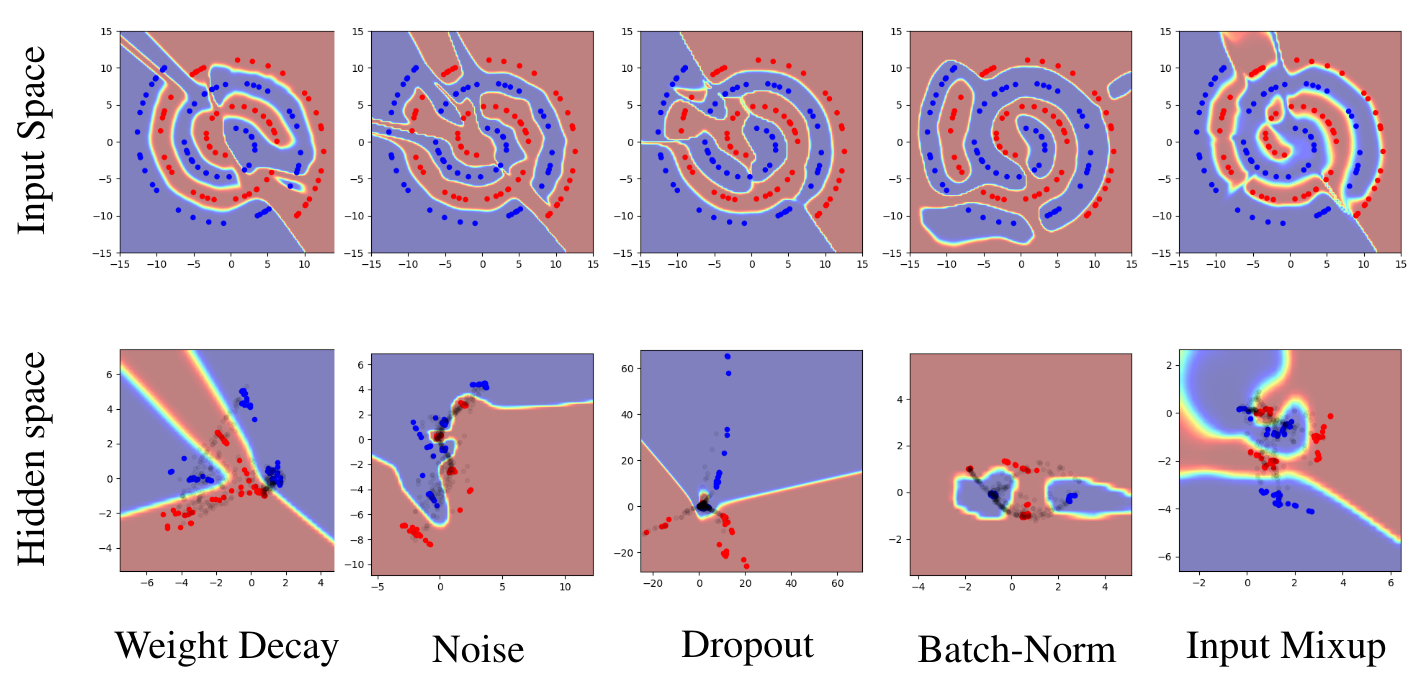
\includegraphics[scale=0.25]{./images/mixup.png}
    \caption{\protect\hypertarget{image10}{Эксперимент с сетью, обученной на 2D наборе спиральных данных с использованием различных регуляризаторов. Эксперимент показывает, что эффект обеспечения широкой области низкой достоверности между областями классов не достигается другими регуляризаторами. Batch Normalization и Dropout на всех слоях, Dropout с вероятностью 0.5, под шумом подразумевается гауссовский шум.
 \\ Взято из \protect\hyperlink{cite.Ver18}{[1]}.}}
\end{figure}

Manifold Mixup улучшает обобщение глубоких нейронных сетей по следующим причинам:
\begin{enumerate}
\item Приводит к более плавным границам принятия решений, которые находятся дальше от обучающих данных, на нескольких уровней пространства признаков. Гладкость и маржа являются общепризнанными факторами генерализации \hyperlink{cite.Pet98}{[28]}.  
\item Использует интерполяцию в более глубоких скрытых слоях, которые собирают информацию более высокого уровня, для обеспечения дополнительного обучающего сигнала.
\item Сглаживает представления классов, значительно сокращая их количество направлений дисперсии (будет описано далее).
\end{enumerate}

\paragraph{Метод}
Рассмотрим обучение глубокой нейронной сети $f(x) = f_k(g_k(x))$, где $g_k$ обозначает часть нейронной сети, отображающую входные данные в скрытое представление на уровне $k$, а $f_k$ обозначает часть, отображающую данное скрытое представление в выход $f(x)$. 

Вначале мы выбираем случайный уровень $k$ из набора допустимых уровней $S$ в нейронной сети. Этот набор может включать в себя самый первый уровень $g_0(x)$. На практике $k$ выбирается равновероятно из некоторых фиксированных уровней.

Далее считается скрытое представление образцов $(x, y)$ и $(x_0, y_0)$ до уровня $k$. После этого есть промежуточные образцы $(g_k(x), y)$ и $(g_k(x_0), y_0)$. На практике $(x, y)$ и $(x_0, y_0)$ берутся из одного батча. Подробности в \hyperref[sec:Chapter3]{Главе 4}.

После слоя $k$ происходит mixup \hyperlink{cite.Hon17}{[25]}:
\begin{equation}
    (\tilde{g_k}, \tilde{y}) = (Mix_{\lambda}(g_k(x), g_k(x_0)), Mix_{\lambda}(y, y_0))
\end{equation}
где $Mix_{\lambda}(a, b) = \lambda \cdot a + (1 - \lambda) \cdot b$. Здесь $(y, y_0)$ - это целевые переменные, а коэффициент $\lambda$ выбирается из распределения $Beta(\alpha, \alpha)$, как и в \hyperlink{cite.Hon17}{[25]}.

Наконец, данное скрытое представление отображается в выход обычным образом и считается функция ошибки.

Формально говоря, Manifold Mixup минимизирует:
\begin{equation}
L(f) = \mathbb{E}_{(x,y) \sim P} \mathbb{E}_{(x_0, y_0) \sim P} \mathbb{E}_{\lambda \sim \text{Beta}(\alpha, \alpha)} \mathbb{E}_{k \sim S} l( f_k\left( \text{Mix}_{\lambda}(g_k(x), g_k(x_0)) \right), \text{Mix}_{\lambda}(y, y_0)).
\end{equation}
где $l$ - функция ошибки, $P$ - распределение входных данных.

\paragraph{Теоретическое обоснование}
Предположим, что $\mathcal{X}$ и $\mathcal{H}$ обозначают пространства входных данных и признаков соответственно. Обозначим целевое множество $\mathcal{Y}$, а $\mathcal{Z} = \mathcal{X} \times \mathcal{Y}$. Пусть $\mathcal{G} \subseteq \mathcal{H}^\mathcal{X}$ обозначает множество функций, реализуемых нейронной сетью, от ввода к данному пространству признаков (до слоя $k$). Аналогично, пусть $\mathcal{F} \subseteq \mathcal{Y}^\mathcal{H}$ будет множеством всех функций, реализуемых нейронной сетью, от представления к ответу. Тогда решение задачи можно описать в следующем виде:

\begin{equation}
J(P) = \inf_{g\in G, f\in F} \mathbb{E}_{(x,y),(x_0, y_0), \lambda} l( f(Mix_\lambda(g(x), g(x_0))), Mix_\lambda(y, y_0))
\end{equation}

Точнее говоря, пусть $P_D$ - эпирическое распределение, $D = \{(x_i, y_i)\}_{i=1}^{n}$. Затем, пусть $f^* \in \mathcal{F}$ и $g^* \in \mathcal{G}$ будут минимизаторами $J(P)$ для $P = P_D$. Также пусть $\mathcal{G} = \mathcal{H}^\mathcal{X}$ и $\mathcal{F} = \mathcal{Y}^\mathcal{H}$, и $\mathcal{H}$ является векторным пространством. Эти условия утверждают, что отображения, реализуемые большими нейронными сетями, плотны во множестве всех непрерывных ограниченных функций. В этом случае мы покажем, что минимизатор $f^*$ является линейной функцией из $\mathcal{H}$ в $\mathcal{Y}$. В таком случае, $J(P)$ может быть переписано следующим образом:

\begin{equation}
J(P_D) = \inf_{h_1,...,h_n \in \mathcal{H}} \frac{1}{n(n-1)} \sum_{i \neq j}^n \inf_{f \in \mathcal{F}} \int_{0
}^{1} l( f(\text{Mix}_{\lambda}(h_i, h_j)), \text{Mix}_{\lambda}(y_i, y_j)) p(\lambda) d\lambda
\end{equation}
где $h_i = g(x_i)$.

\begin{theorem}
Пусть $\mathcal{H}$ - векторное пространство размерности $dim(\mathcal{H})$, и пусть $d \in \mathbb{N}$ обозначает количество классов, содержащихся в датасете $D$. Если $dim (\mathcal{H}) \geq d-1$, то $J(P_D) = 0$ и соответствующий минимизатор $f^*: \mathcal{H} \rightarrow \mathbb{R}^d$ является линейной функцией.
\end{theorem}
\begin{proof}
Сначала заметим, что если $dim(\mathcal{H}) \geq d - 1$, то:
$$ \exists A, H \in \mathbb{R}^{dim(\mathcal{H}) \times d}, b \in \mathbb{R}^{d}: A^T H + b1_{d}^T = I_{d \times d}, $$
где $I_{d \times d}$ и $1_d$ обозначают $d$-мерную единичную матрицу и вектор из единиц соответственно. Фактически,
$b1_{d}^T$ является матрицей ранга один, тогда как ранг единичной матрицы равен $d$. Таким образом, для $A^T H$ достаточно только ранга $d - 1$.

Пусть $f^{*}(h) = A^T h + b$ для всех $h \in \mathcal{H}$. Пусть $g^{*}(x_i) = H_{\zeta_i,:}$ пусть $\zeta_i$-м столбцом матрицы $H$, где
$\zeta_i \in \{1, , d\}$ обозначает индекс класса примера xi. Эти выборы минимизируют (2), так как:
$$ `(f^?(Mix\lambda(g^?(xi), g^?(xj))), Mix\lambda(yi, yj)) = `(A^T Mix\lambda(H{\zeta_i,:}, H{\zeta_j,:}) + b, Mix\lambda(y{i,\zeta_i}, y{j,\zeta_j})) = `(u, u) = 0. $$
Результат следует из $A^T H{\zeta_i,:} + b = y{i,\zeta_i}$ для всех i.
\end{proof}

\paragprah Адаптация к Connectionist temporal classification


\newpage %% Обзор существующих решений
    \section{Конфигурация}
\label{sec:Chapter3} \index{Chapter3}

\begin{figure}
    \centering
    Real \\
    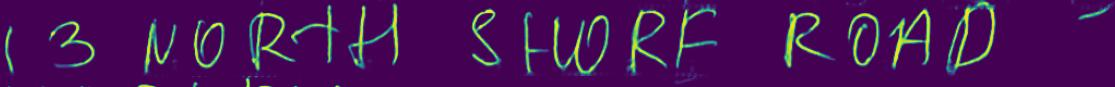
\includegraphics[scale=0.45]{./images/data/Real.jpg} \\
    Synthetic
    \\
    
\includegraphics[scale=3]{./images/data/Synthetic.jpg} \\
    SynForms
    \\
    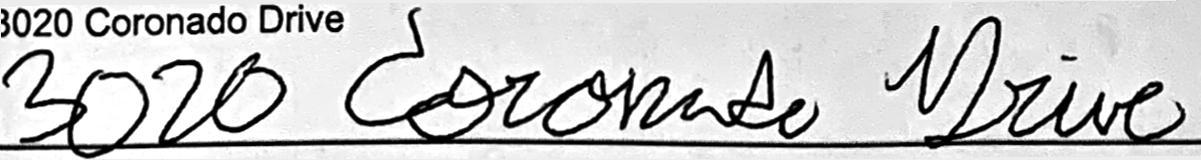
\includegraphics[scale=0.4]{./images/data/SynForms.jpg}
    \caption{\protect\hypertarget{image11}{Примеры изображений из датасета.}}
\end{figure}

\subsection{Описание модели}
В качестве энкодера использовался TransformerEncoder с следующими параметрами:
\begin{enumerate}
\item количество слоев: $6$
\item nhead в multiheadattention): $4$
\item размерномть feedforward сети: $768$
\item размерность пространства признаков: $128$
\end{enumerate}

В качестве сверточной нейронной сети для извлечения визуальных признаков использовался ResNet \hyperlink{cite.Kai15}{[17]}. В качестве функции активации использовалась ReLU. Далее архитектура ResNet описывается чуть подробнее:

\subsubsection{ConvBN}
Слой ConvBN представляет из себя композицию свертки (conv) и батч-нормализации (BN). Параметры BN следующие:
\begin{enumerate}
\item eps: $10^{-12}$
\item momentum: $0.01$
\end{enumerate}
За filters будем обозначать количество фильтров свертки. За kernel размер ядра, padding и stride также есть соответсвующие параметры свертки.

\subsubsection{ResNetBlock}
Этот residual блок предстваляет из себя композицию трех ConvBN (с размерами ядра: $[1, 3, 1]$, padding: $[0, 1, 0]$). Функция активации: ReLU (как было сказано ранее).

\subsubsection{FeatureBlock}
Это композиция нескольких ResNetBlock. Также для всех FeatureBlock, кроме последнего, после ResNetBlock-ов есть еще ConvBN слой (kernel: $3$, padding: $1$). В некоторых случаях (кроме последних двух) данный блок завершается max-pool (kernel: $2$). После FeatureBlock для регуляризации использовался dropout \hyperlink{cite.Sut14}{[12]} (с вероятностью $0.1$).

Первый FeatureBlock отличается от остальных: он представляет из себя композицию двух ConvBN (kernel: $[3, 3]$, padding: $[1, 1]$) и max-pool (kernel: $2$) слоя.

\paragraph{}

ResNet преставляет из себя композицию нескольких FeatureBlock-ов (всего $5$, с количествами ResNetBlock: $[1, 2, 5, 3]$, первый FeatureBlock отличается от остальных). После FeatureBlock-ов идут два ConvBN и dropout (c вероятностью $0.2$). 


\subsection{Описание датасета}

Данные можно разделить на три категории:
\begin{enumerate}
\item Real: Данные, собранные с документов. Обычно это поля различных контрактов, форм, или поля на счетах
\item SynForms: Написанные людьми строки текста
\item Synthetic: Псевдорукописные шрифты после применения некоторых аугментаций
\end{enumerate}
Примеры изображений можно найти на \hyperlink{image11}{[Рис 11.]}. Для обучения брались данные из всех трех групп в соотношении $1:1:1$.

\begin{figure}
    \centering
    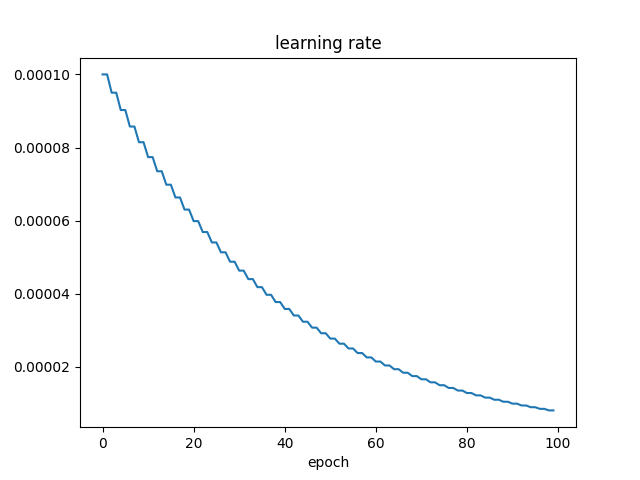
\includegraphics[scale=0.5]{./images/lr.png} 
    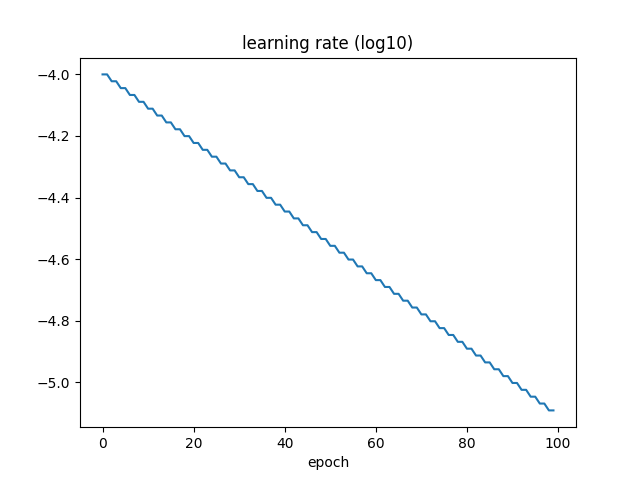
\includegraphics[scale=0.5]{./images/lr_log.png}
    \caption{\protect\hypertarget{image12}{Как менялся learning rate во время обучения.}}
\end{figure}

\subsection{Оптимизатор}
В качестве оптимизатора использовался AdamW \hyperlink{cite.Los17}{[29]} с параметрами:
\begin{enumerate}
\item betas: $(0.9, 0.999)$
\item weight decay: $0.01$
\end{enumerate}
Learning rate начинался с $0.0001$ и умножался на $0.95$ каждые две эпохи \hyperlink{image12}{[Рис 12.]}. Также во всех экспериментах размер батча был равен $64$. Использовалась точность \href{https://pytorch.org/blog/what-every-user-should-know-about-mixed-precision-training-in-pytorch/}{mixed precision в PyTorch}. Также, если не сказано иного, обучение ведется в течение $100$ эпох.

\subsection{Реализация mixup}
Для более эффективной работы, образцы $(x, y)$ и $(x_0, y_0)$ семплируются каждый раз внутри одного батча. Точнее говоря, если мы имеем батч $(x_1, \dots, x_N)$, то операция mixup выглядит следующим образом:

\begin{equation}
\begin{split}
y_{1:N} = shuffle(x_{1:N}) \\
\tilde{x}_{1:N} = \lambda x_{1:N} + (1 - \lambda) y_{1:N}
\end{split}
\end{equation}

Основываясь на результатах \hyperlink{cite.Bas19}{[16]}, по умолчанию (если не сказано иного) $\alpha = 0.5$, то есть $\lambda \sim Beta(0.5, 0.5)$. Каждый раз, во время обучения, mixup происходит лишь в одной позиции. Эта позиция выбирается случайно из набора.



\newpage %% Исследование и построение решения задачи
    \section{Результаты экспериментов}
\label{sec:Chapter4} \index{Chapter4}

Если в рамках работы писался какой-то код, здесь должно быть его
описание: выбранный язык и библиотеки и мотивы выбора, архитектура,
схема функционирования, теоретическая сложность алгоритма, характеристики
функционирования (скорость/память).

\newpage
 %% Описание практической части
    \section{Вывод}
\label{sec:Chapter5} \index{Chapter5}

В этой работе исследована стратегия обучения модели с attention-энкодером для задачи распознавания рукописного текста. Предложен метод применения manifold mixup к изображениям разного размера с использованием Connectionist Temporal Classification. Анализируется влияние manifold mixup на процесс обучения нейронной сети. Также исследованы различные аспекты метода, такие как влияние выбора позиции. 

Доказано, что этот метод действует как сильный регуляризатор. Продемонстрировано значительное улучшение результатов распознавания текста \hyperref[tab:mixup_size_max]{[Таблица 1]}. 

В результате экспериментов были обнаружены следующие свойства подхода mixup:
\begin{enumerate}
\item Mixup действует как сильный регуляризатор. В частности, функция ошибки на валидационной выборке достигает некоторой горизонтальной асимптоты, в то время как без mixup модель переобучается и функция ошибки начинает расти.
\item Mixup замедляет обучение на ранних эпохах. В частности, требуется некоторое количество эпох, чтобы функция ошибки и другие метрики начали превосходить результаты модели без mixup.
\item Mixup показывает улучшение всех метрик и функции ошибки при всех наборах позиций. Тем не менее, выбор набора влияет на результаты.
В связи с этим рекомендуется при использовании mixup проводить обучение в течение достаточного количества эпох (возможно дольше в сравнении с обучением без mixup), а также грамотно выбирать набор позиций (например, проводя эксперименты на небольшом количестве данных).
\end{enumerate}
\newpage %% Заключение

    %% НЕ ТРОГАЙТЕ!!!
    \nocite{*}
    \bibliography{references}

    %% в зависимости от надобности подключаем раздел "Приложение"
    % \newpage
    % \section*{Приложение}
\addcontentsline{toc}{section}{Приложение}
\label{sec:Apendix} \index{Apendix}

\subsection{Позиция mixup}

\begin{longtable}{cccc}
\centering
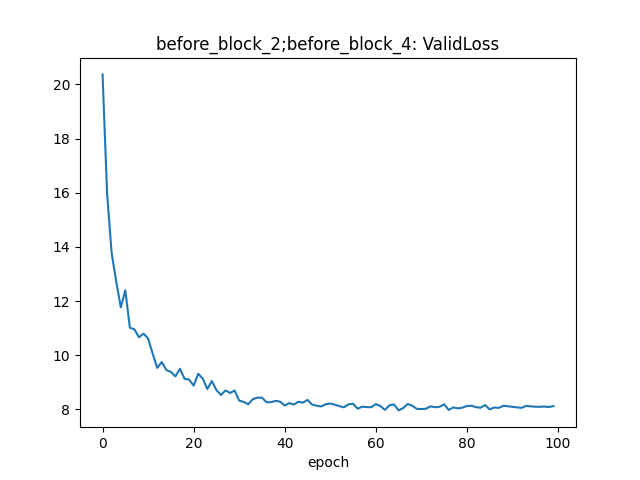
\includegraphics[scale=0.2]{./images/mixup_position/before_block_2;before_block_4_ValidLoss.png} & 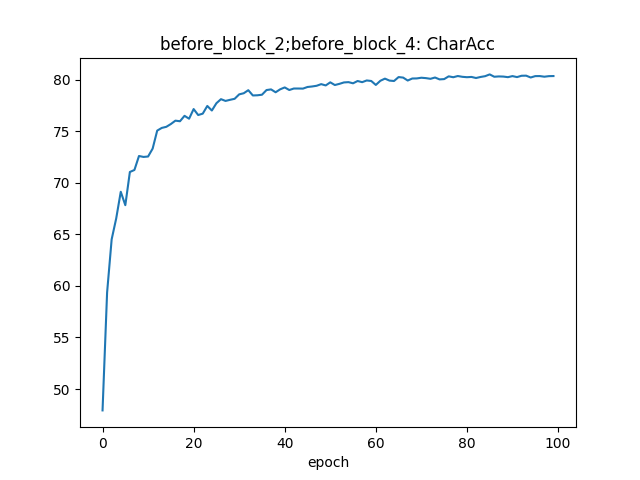
\includegraphics[scale=0.2]{./images/mixup_position/before_block_2;before_block_4_CharAcc.png} & 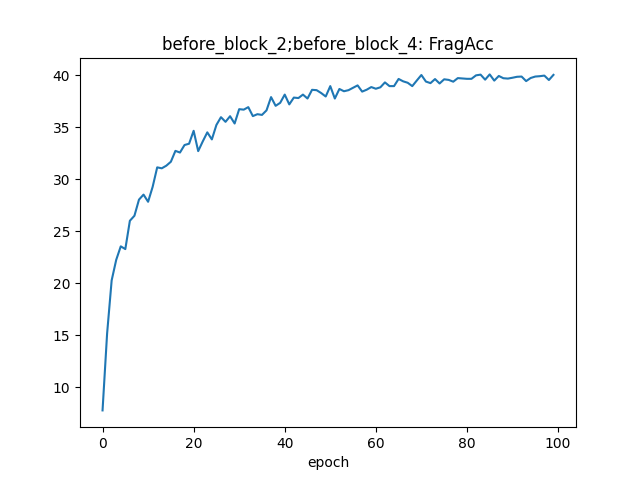
\includegraphics[scale=0.2]{./images/mixup_position/before_block_2;before_block_4_FragAcc.png} & 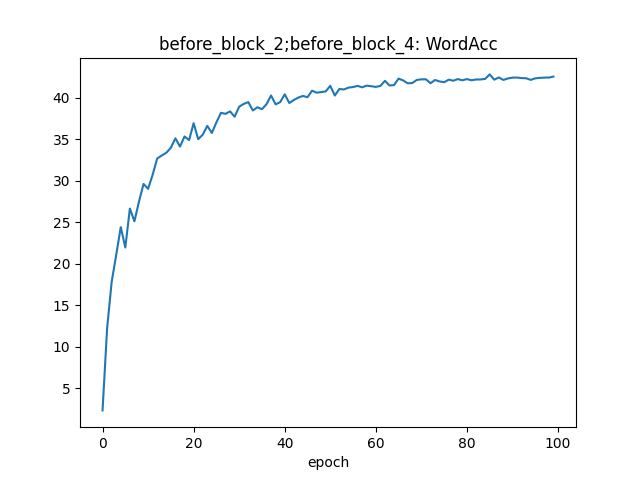
\includegraphics[scale=0.2]{./images/mixup_position/before_block_2;before_block_4_WordAcc.png}\\
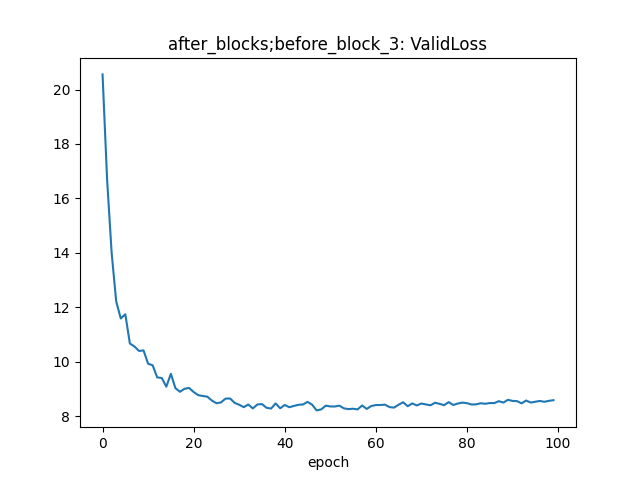
\includegraphics[scale=0.2]{./images/mixup_position/after_blocks;before_block_3_ValidLoss.png} & 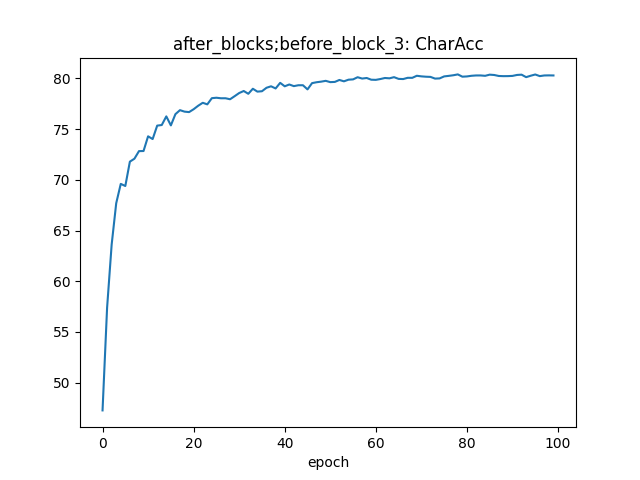
\includegraphics[scale=0.2]{./images/mixup_position/after_blocks;before_block_3_CharAcc.png} & 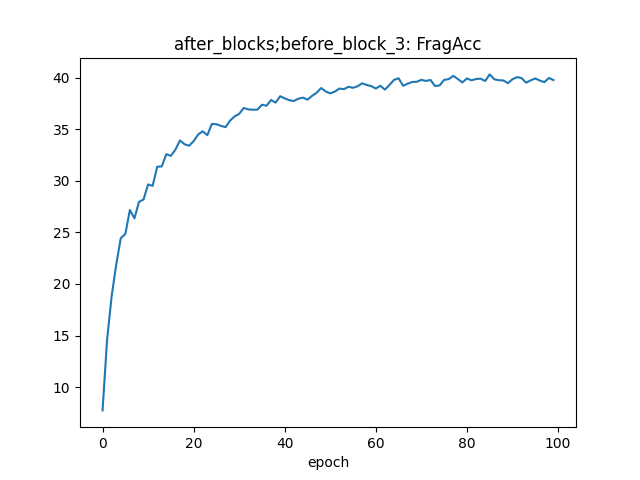
\includegraphics[scale=0.2]{./images/mixup_position/after_blocks;before_block_3_FragAcc.png} & 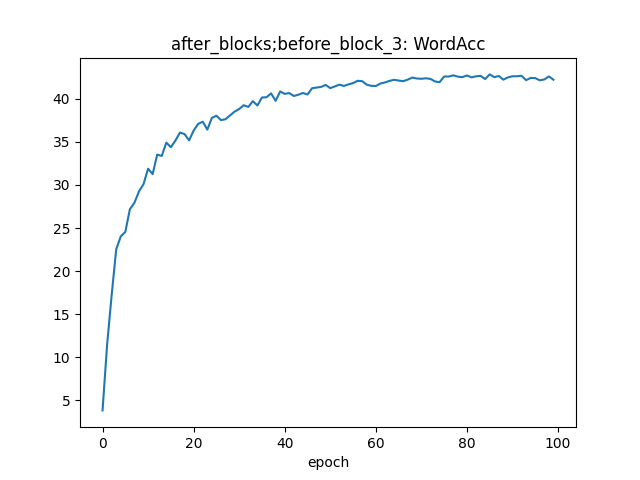
\includegraphics[scale=0.2]{./images/mixup_position/after_blocks;before_block_3_WordAcc.png}\\
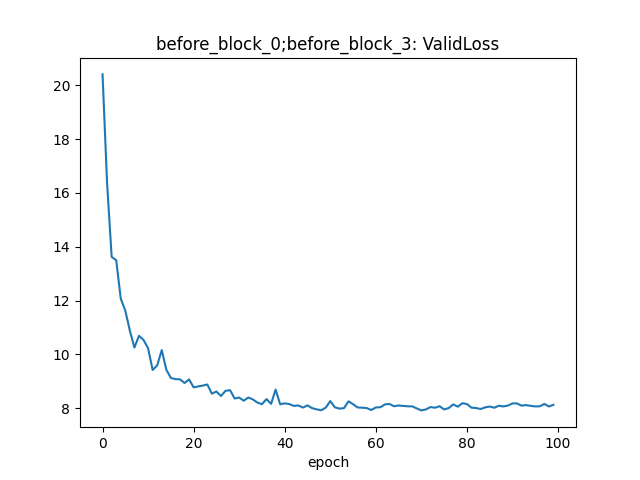
\includegraphics[scale=0.2]{./images/mixup_position/before_block_0;before_block_3_ValidLoss.png} & 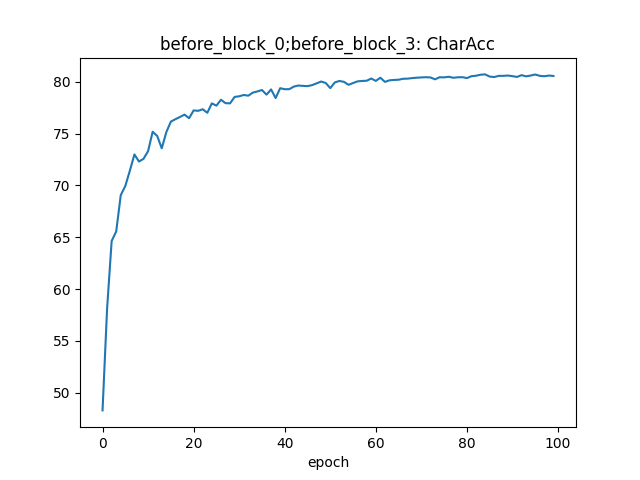
\includegraphics[scale=0.2]{./images/mixup_position/before_block_0;before_block_3_CharAcc.png} & 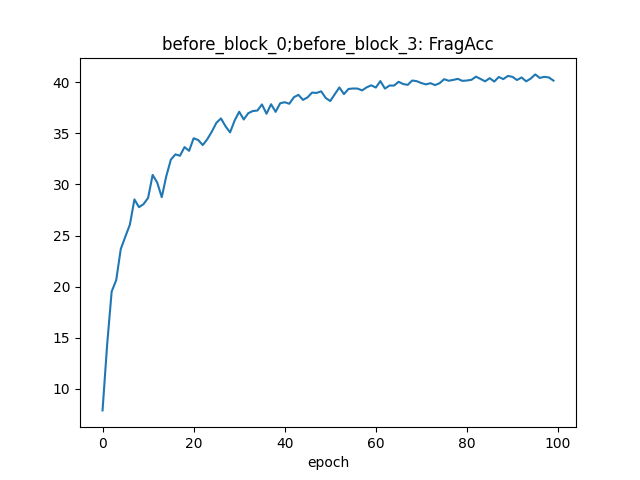
\includegraphics[scale=0.2]{./images/mixup_position/before_block_0;before_block_3_FragAcc.png} & 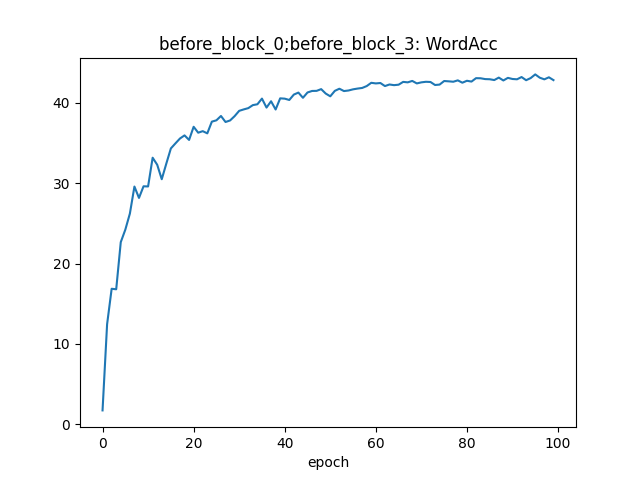
\includegraphics[scale=0.2]{./images/mixup_position/before_block_0;before_block_3_WordAcc.png}\\
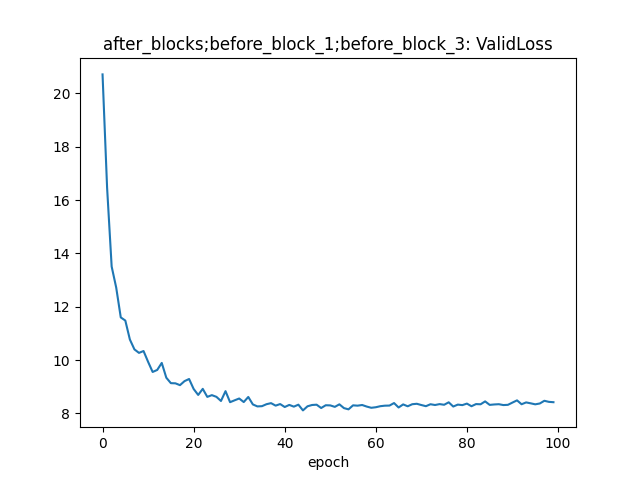
\includegraphics[scale=0.2]{./images/mixup_position/after_blocks;before_block_1;before_block_3_ValidLoss.png} & 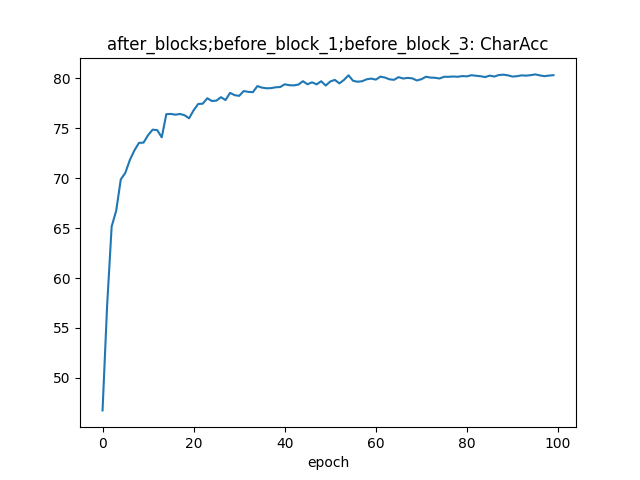
\includegraphics[scale=0.2]{./images/mixup_position/after_blocks;before_block_1;before_block_3_CharAcc.png} & 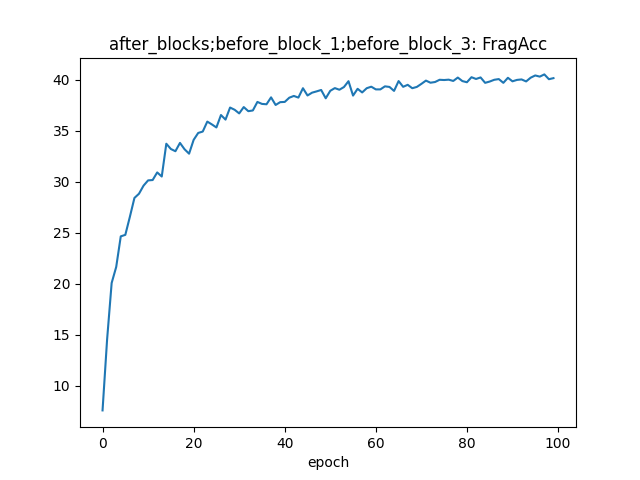
\includegraphics[scale=0.2]{./images/mixup_position/after_blocks;before_block_1;before_block_3_FragAcc.png} & 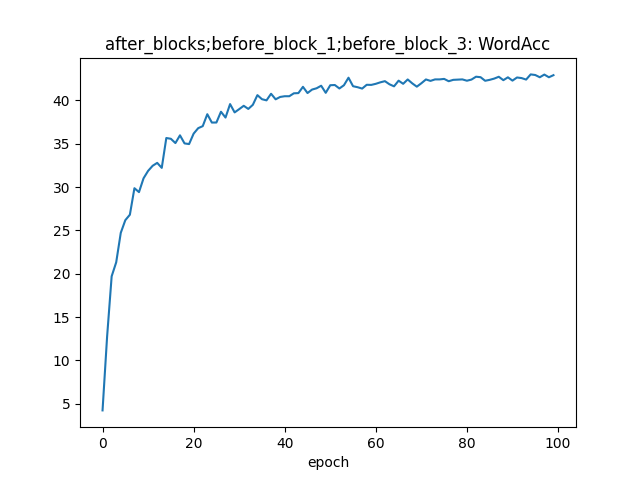
\includegraphics[scale=0.2]{./images/mixup_position/after_blocks;before_block_1;before_block_3_WordAcc.png}\\
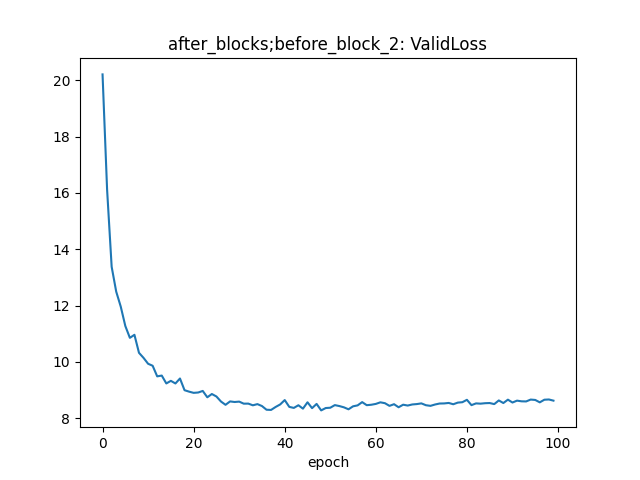
\includegraphics[scale=0.2]{./images/mixup_position/after_blocks;before_block_2_ValidLoss.png} & 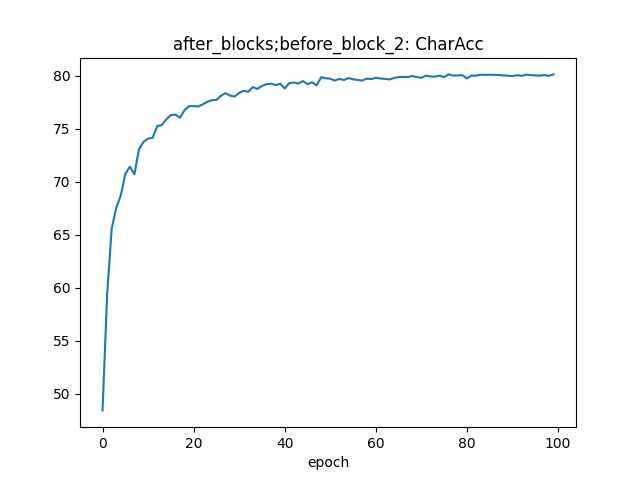
\includegraphics[scale=0.2]{./images/mixup_position/after_blocks;before_block_2_CharAcc.png} & 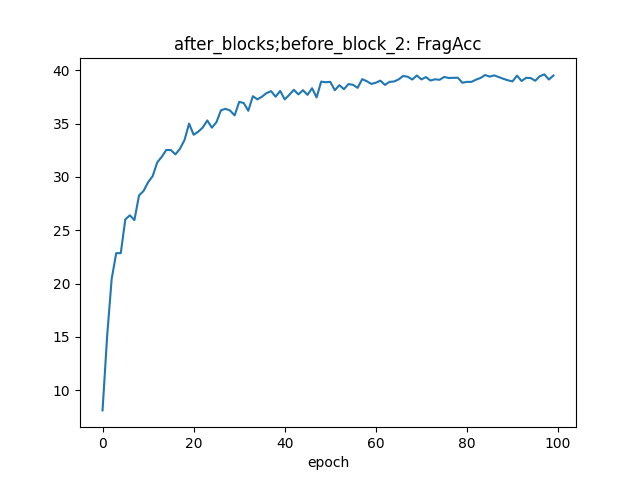
\includegraphics[scale=0.2]{./images/mixup_position/after_blocks;before_block_2_FragAcc.png} & 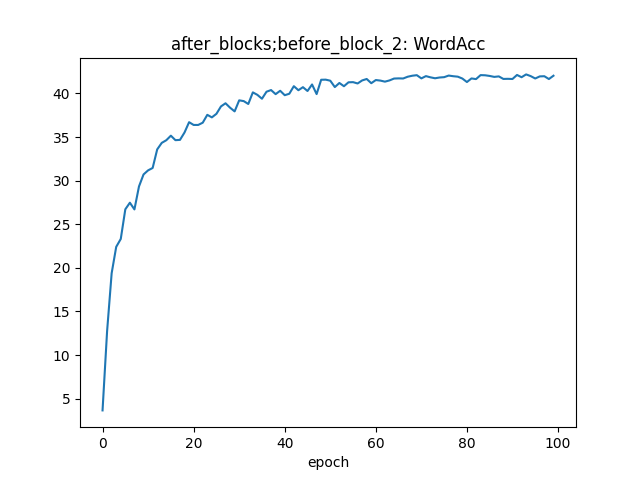
\includegraphics[scale=0.2]{./images/mixup_position/after_blocks;before_block_2_WordAcc.png}\\
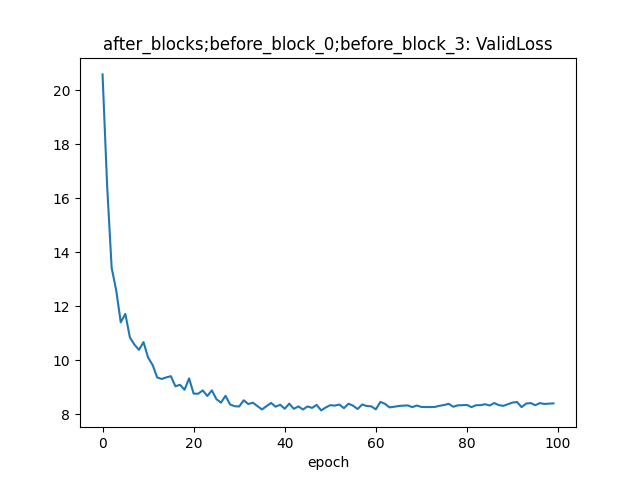
\includegraphics[scale=0.2]{./images/mixup_position/after_blocks;before_block_0;before_block_3_ValidLoss.png} & 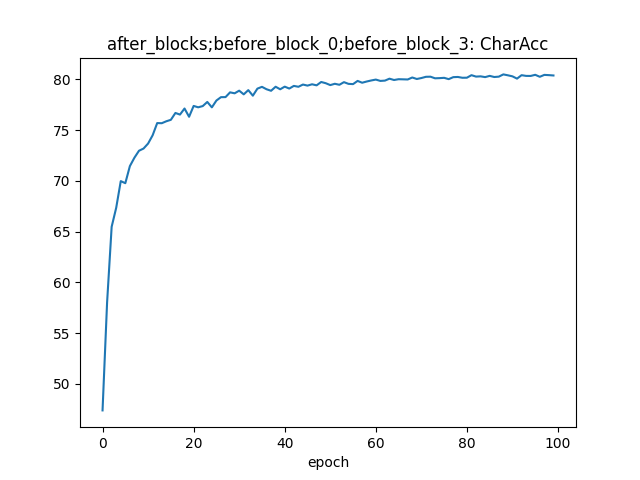
\includegraphics[scale=0.2]{./images/mixup_position/after_blocks;before_block_0;before_block_3_CharAcc.png} & 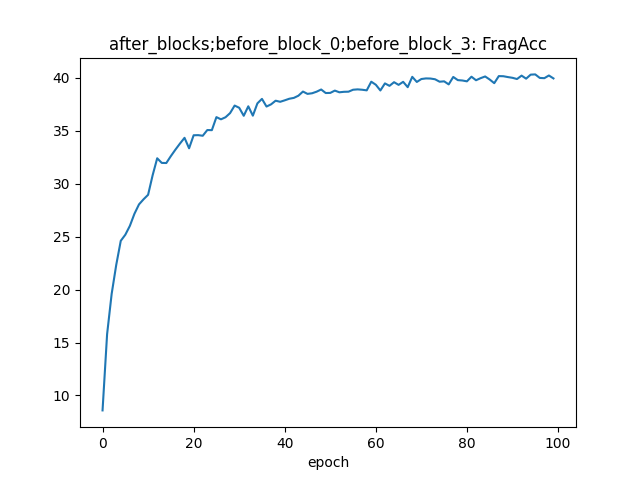
\includegraphics[scale=0.2]{./images/mixup_position/after_blocks;before_block_0;before_block_3_FragAcc.png} & 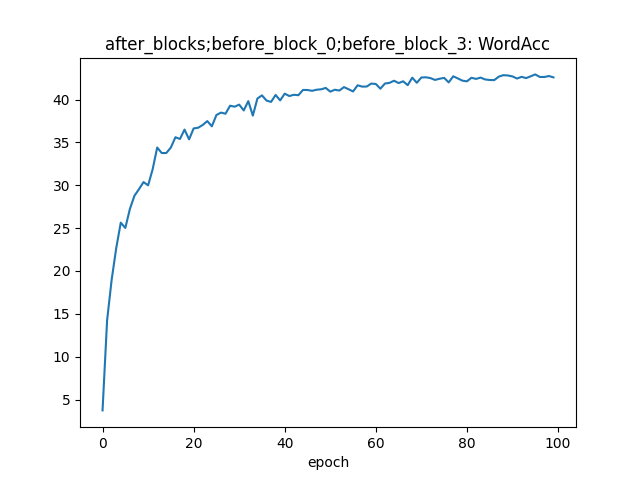
\includegraphics[scale=0.2]{./images/mixup_position/after_blocks;before_block_0;before_block_3_WordAcc.png}\\
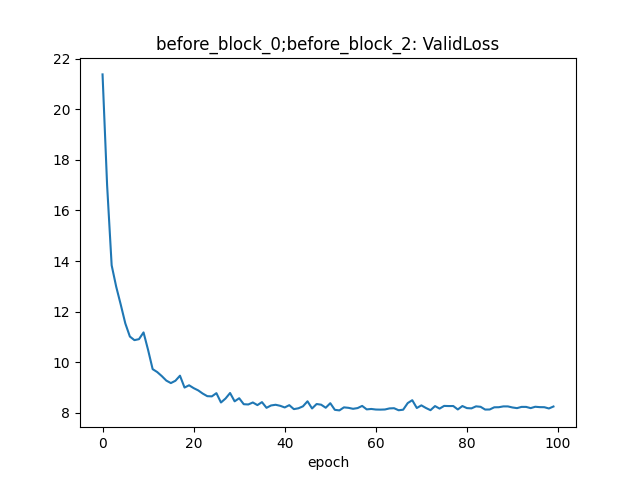
\includegraphics[scale=0.2]{./images/mixup_position/before_block_0;before_block_2_ValidLoss.png} & 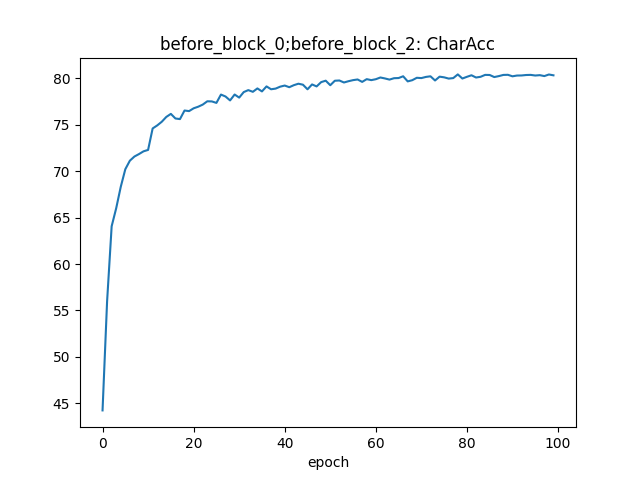
\includegraphics[scale=0.2]{./images/mixup_position/before_block_0;before_block_2_CharAcc.png} & 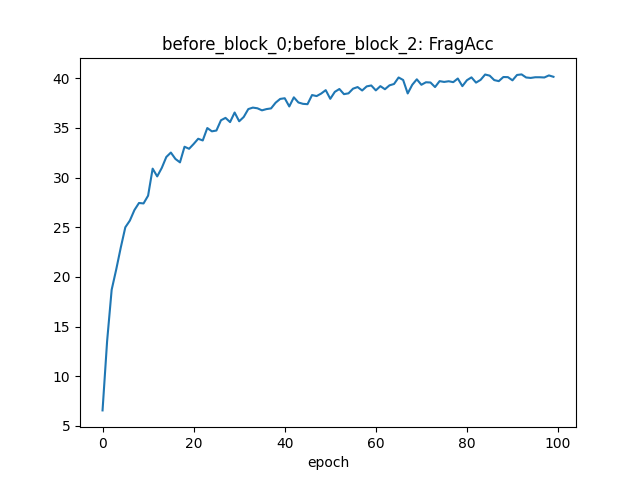
\includegraphics[scale=0.2]{./images/mixup_position/before_block_0;before_block_2_FragAcc.png} & 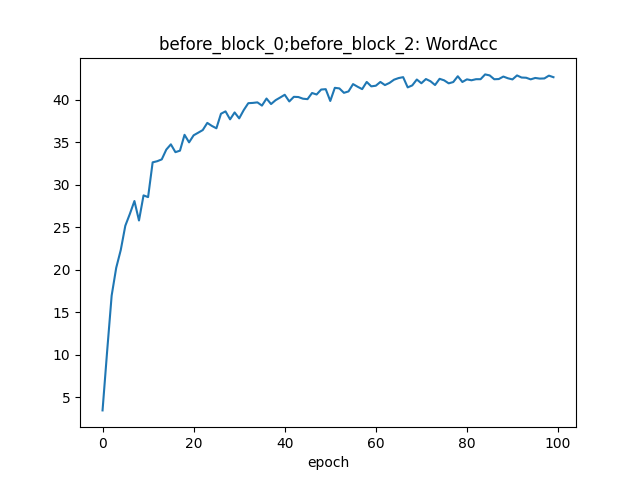
\includegraphics[scale=0.2]{./images/mixup_position/before_block_0;before_block_2_WordAcc.png}\\
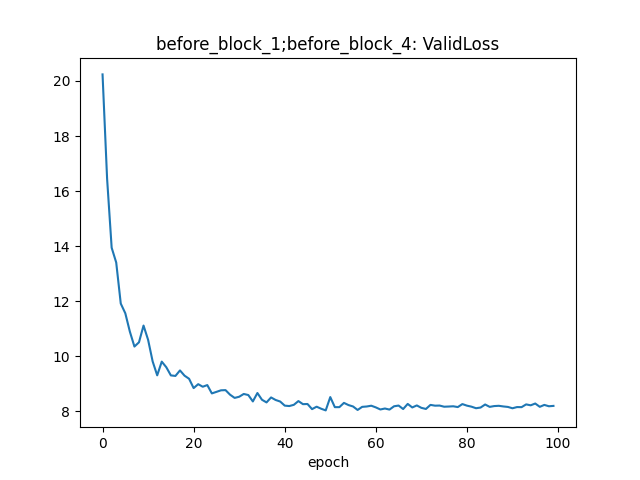
\includegraphics[scale=0.2]{./images/mixup_position/before_block_1;before_block_4_ValidLoss.png} & 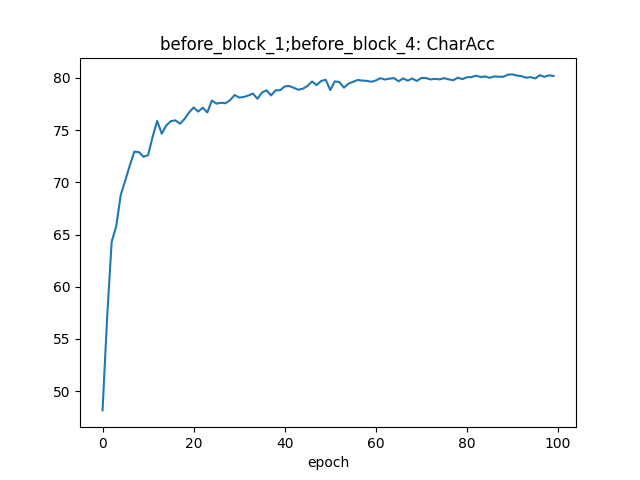
\includegraphics[scale=0.2]{./images/mixup_position/before_block_1;before_block_4_CharAcc.png} & 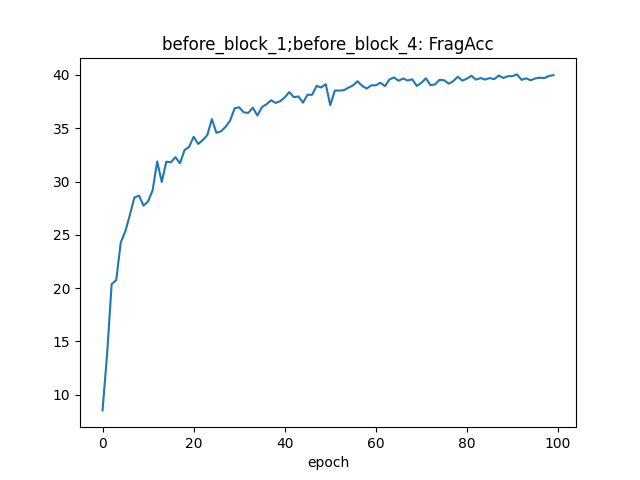
\includegraphics[scale=0.2]{./images/mixup_position/before_block_1;before_block_4_FragAcc.png} & 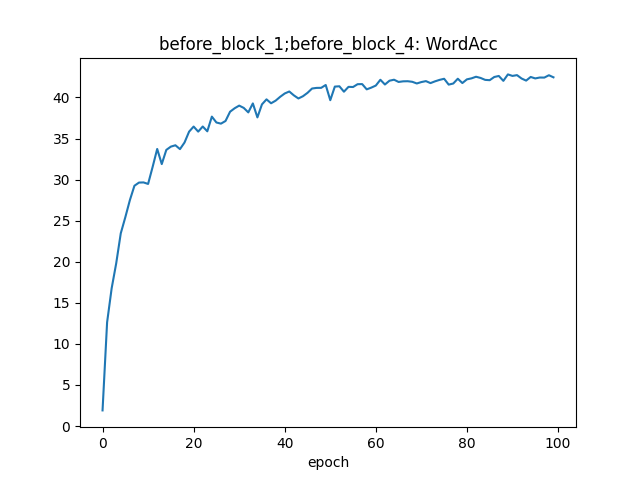
\includegraphics[scale=0.2]{./images/mixup_position/before_block_1;before_block_4_WordAcc.png}\\
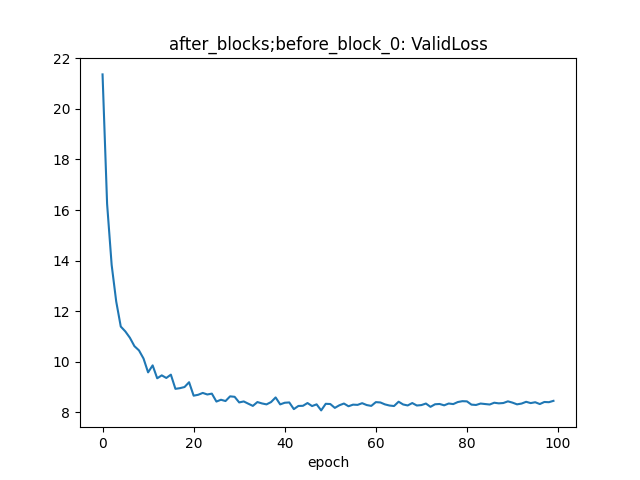
\includegraphics[scale=0.2]{./images/mixup_position/after_blocks;before_block_0_ValidLoss.png} & \includegraphics[scale=0.2]{./images/mixup_position/after_blocks;before_block_0_CharAcc.png} & \includegraphics[scale=0.2]{./images/mixup_position/after_blocks;before_block_0_FragAcc.png} & \includegraphics[scale=0.2]{./images/mixup_position/after_blocks;before_block_0_WordAcc.png}\\
\includegraphics[scale=0.2]{./images/mixup_position/after_final_conv1;before_block_1;before_block_4_ValidLoss.png} & \includegraphics[scale=0.2]{./images/mixup_position/after_final_conv1;before_block_1;before_block_4_CharAcc.png} & \includegraphics[scale=0.2]{./images/mixup_position/after_final_conv1;before_block_1;before_block_4_FragAcc.png} & \includegraphics[scale=0.2]{./images/mixup_position/after_final_conv1;before_block_1;before_block_4_WordAcc.png}\\
\includegraphics[scale=0.2]{./images/mixup_position/before_block_0;before_block_4_ValidLoss.png} & \includegraphics[scale=0.2]{./images/mixup_position/before_block_0;before_block_4_CharAcc.png} & \includegraphics[scale=0.2]{./images/mixup_position/before_block_0;before_block_4_FragAcc.png} & \includegraphics[scale=0.2]{./images/mixup_position/before_block_0;before_block_4_WordAcc.png}\\
\includegraphics[scale=0.2]{./images/mixup_position/after_blocks;before_block_1_ValidLoss.png} & \includegraphics[scale=0.2]{./images/mixup_position/after_blocks;before_block_1_CharAcc.png} & \includegraphics[scale=0.2]{./images/mixup_position/after_blocks;before_block_1_FragAcc.png} & \includegraphics[scale=0.2]{./images/mixup_position/after_blocks;before_block_1_WordAcc.png}\\
\includegraphics[scale=0.2]{./images/mixup_position/after_final_conv1;before_block_2;before_block_4_ValidLoss.png} & \includegraphics[scale=0.2]{./images/mixup_position/after_final_conv1;before_block_2;before_block_4_CharAcc.png} & \includegraphics[scale=0.2]{./images/mixup_position/after_final_conv1;before_block_2;before_block_4_FragAcc.png} & \includegraphics[scale=0.2]{./images/mixup_position/after_final_conv1;before_block_2;before_block_4_WordAcc.png}\\
\includegraphics[scale=0.2]{./images/mixup_position/after_final_conv1;before_block_3_ValidLoss.png} & \includegraphics[scale=0.2]{./images/mixup_position/after_final_conv1;before_block_3_CharAcc.png} & \includegraphics[scale=0.2]{./images/mixup_position/after_final_conv1;before_block_3_FragAcc.png} & \includegraphics[scale=0.2]{./images/mixup_position/after_final_conv1;before_block_3_WordAcc.png}\\
\includegraphics[scale=0.2]{./images/mixup_position/before_block_0;before_block_2;before_block_4_ValidLoss.png} & \includegraphics[scale=0.2]{./images/mixup_position/before_block_0;before_block_2;before_block_4_CharAcc.png} & \includegraphics[scale=0.2]{./images/mixup_position/before_block_0;before_block_2;before_block_4_FragAcc.png} & \includegraphics[scale=0.2]{./images/mixup_position/before_block_0;before_block_2;before_block_4_WordAcc.png}\\
\includegraphics[scale=0.2]{./images/mixup_position/after_final_conv1;before_block_0;before_block_4_ValidLoss.png} & \includegraphics[scale=0.2]{./images/mixup_position/after_final_conv1;before_block_0;before_block_4_CharAcc.png} & \includegraphics[scale=0.2]{./images/mixup_position/after_final_conv1;before_block_0;before_block_4_FragAcc.png} & \includegraphics[scale=0.2]{./images/mixup_position/after_final_conv1;before_block_0;before_block_4_WordAcc.png}\\
\includegraphics[scale=0.2]{./images/mixup_position/after_final_conv1;before_block_1_ValidLoss.png} & \includegraphics[scale=0.2]{./images/mixup_position/after_final_conv1;before_block_1_CharAcc.png} & \includegraphics[scale=0.2]{./images/mixup_position/after_final_conv1;before_block_1_FragAcc.png} & \includegraphics[scale=0.2]{./images/mixup_position/after_final_conv1;before_block_1_WordAcc.png}\\
\includegraphics[scale=0.2]{./images/mixup_position/after_final_conv1;before_block_0_ValidLoss.png} & \includegraphics[scale=0.2]{./images/mixup_position/after_final_conv1;before_block_0_CharAcc.png} & \includegraphics[scale=0.2]{./images/mixup_position/after_final_conv1;before_block_0_FragAcc.png} & \includegraphics[scale=0.2]{./images/mixup_position/after_final_conv1;before_block_0_WordAcc.png}\\
\includegraphics[scale=0.2]{./images/mixup_position/after_final_conv1;before_block_0;before_block_2_ValidLoss.png} & \includegraphics[scale=0.2]{./images/mixup_position/after_final_conv1;before_block_0;before_block_2_CharAcc.png} & \includegraphics[scale=0.2]{./images/mixup_position/after_final_conv1;before_block_0;before_block_2_FragAcc.png} & \includegraphics[scale=0.2]{./images/mixup_position/after_final_conv1;before_block_0;before_block_2_WordAcc.png}\\
\includegraphics[scale=0.2]{./images/mixup_position/_ValidLoss.png} & \includegraphics[scale=0.2]{./images/mixup_position/_CharAcc.png} & \includegraphics[scale=0.2]{./images/mixup_position/_FragAcc.png} & \includegraphics[scale=0.2]{./images/mixup_position/_WordAcc.png}\\
\includegraphics[scale=0.2]{./images/mixup_position/after_final_conv1;before_block_2_ValidLoss.png} & \includegraphics[scale=0.2]{./images/mixup_position/after_final_conv1;before_block_2_CharAcc.png} & \includegraphics[scale=0.2]{./images/mixup_position/after_final_conv1;before_block_2_FragAcc.png} & \includegraphics[scale=0.2]{./images/mixup_position/after_final_conv1;before_block_2_WordAcc.png}\\
\includegraphics[scale=0.2]{./images/mixup_position/after_final_conv1;before_block_1;before_block_3_ValidLoss.png} & \includegraphics[scale=0.2]{./images/mixup_position/after_final_conv1;before_block_1;before_block_3_CharAcc.png} & \includegraphics[scale=0.2]{./images/mixup_position/after_final_conv1;before_block_1;before_block_3_FragAcc.png} & \includegraphics[scale=0.2]{./images/mixup_position/after_final_conv1;before_block_1;before_block_3_WordAcc.png}\\
\includegraphics[scale=0.2]{./images/mixup_position/after_final_conv1;before_block_0;before_block_3_ValidLoss.png} & \includegraphics[scale=0.2]{./images/mixup_position/after_final_conv1;before_block_0;before_block_3_CharAcc.png} & \includegraphics[scale=0.2]{./images/mixup_position/after_final_conv1;before_block_0;before_block_3_FragAcc.png} & \includegraphics[scale=0.2]{./images/mixup_position/after_final_conv1;before_block_0;before_block_3_WordAcc.png}\\
\includegraphics[scale=0.2]{./images/mixup_position/after_blocks;before_block_0;before_block_2_ValidLoss.png} & \includegraphics[scale=0.2]{./images/mixup_position/after_blocks;before_block_0;before_block_2_CharAcc.png} & \includegraphics[scale=0.2]{./images/mixup_position/after_blocks;before_block_0;before_block_2_FragAcc.png} & \includegraphics[scale=0.2]{./images/mixup_position/after_blocks;before_block_0;before_block_2_WordAcc.png}\\
\includegraphics[scale=0.2]{./images/mixup_position/before_block_1;before_block_3_ValidLoss.png} & \includegraphics[scale=0.2]{./images/mixup_position/before_block_1;before_block_3_CharAcc.png} & \includegraphics[scale=0.2]{./images/mixup_position/before_block_1;before_block_3_FragAcc.png} & \includegraphics[scale=0.2]{./images/mixup_position/before_block_1;before_block_3_WordAcc.png}\\
\includegraphics[scale=0.2]{./images/mixup_position/after_final_conv1;before_block_4_ValidLoss.png} & \includegraphics[scale=0.2]{./images/mixup_position/after_final_conv1;before_block_4_CharAcc.png} & \includegraphics[scale=0.2]{./images/mixup_position/after_final_conv1;before_block_4_FragAcc.png} & \includegraphics[scale=0.2]{./images/mixup_position/after_final_conv1;before_block_4_WordAcc.png}\\
\caption{Графики функции ошибки и некоторых метрик для каждого варианта позиций mixup.}
\label{tab:mixup_position}
\end{longtable}
\end{document}
